\section{Analiza}

 W~rozdziale zostały przedstawione wyniki przeprowadzonych testów. Dane zostały przedstawione w~tabelach oraz za pomocą wykresów. Każdy z~rezultatów testów został zanalizowany i~opisany.

\subsection{Testy zapisu danych}
 W~podrozdziale zostały przedstawione wyniki testów zapisu danych. Dodatkowo przedstawiono ilość wykorzystanej pamięci operacyjnej podczas operacji oraz stopień wykorzystania procesora. W~systemie iOS nie istnieje możliwość odczytania zajętości pamięci operacyjnej i~zużycia procesora jedynie dla danej operacji. Przedstawione dane pokazują więc parametry dla całej działającej aplikacji. Wyniki te są jak najbardziej miarodajne, gdyż każdy z~testów odbywał się na ''świeżo,, uruchomionej aplikacji i~użycie pamięci operacyjnej i~procesora zawsze miało stały punkt startowy. 

\subsubsection{Mały zestaw danych}

Prezentacja danych w~formie tabel: 

\begin{table}[h]
\centering
\caption{Czasy zapisu danych do bazy - mały zestaw danych}
\label{tab: small-save-time-table}
\begin{tabular}{|c|c|}
\hline
Baza danych   & Czas zapisu [ms] \\ \hline
User Defaults & 2,07             \\ \hline
Realm         & 5,52             \\ \hline
Core Data     & 16,05            \\ \hline
FMDB          & 173,63           \\ \hline
SQLite        & 175,45           \\ \hline
\end{tabular}
\end{table}

\begin{table}[h]
\centering
\caption{Rozmiar pliku wynikowego bazy danych - mały zestaw danych}
\label{tab: small-save-file-size-table}
\begin{tabular}{|c|c|}
\hline
Baza danych   & Rozmiar pliku bazy danych [kb] \\ \hline
User Defaults & 0,04                            \\ \hline
Realm         & 16,38                           \\ \hline
FMDB          & 61,23                           \\ \hline
SQLite        & 61,32                           \\ \hline
Core Data     & 80,04                           \\ \hline
\end{tabular}
\end{table}

\newpage

\begin{table}[h]
\centering
\caption{Użycie procesora podczas operacji - mały zestaw danych}
\label{tab: small-save-cpu-table}
\begin{tabular}{|c|c|}
\hline
Baza danych   & Użycie procesora [\%] \\ \hline
SQLite        & 18                   \\ \hline
FMDB          & 19                   \\ \hline
Realm         & 47                   \\ \hline
Core Data     & 83                   \\ \hline
User Defaults & 88                   \\ \hline
\end{tabular}
\end{table}

\begin{table}[h]
\centering
\caption{Użycie pamięci operacyjnej podczas operacji - mały zestaw danych}
\label{tab: small-save-ram-table}
\begin{tabular}{|c|c|}
\hline
Baza danych   & Użycie pamięci RAM [mb] \\ \hline
User Defaults & 86,4                    \\ \hline
FMDB          & 86,4                    \\ \hline
SQLite        & 86,5                    \\ \hline
Core Data     & 88,6                    \\ \hline
Realm         & 89,7                    \\ \hline
\end{tabular}
\end{table}

\newpage
Prezentacja wyników w~formie wykresów: 

\begin{figure}[h]
\centering
	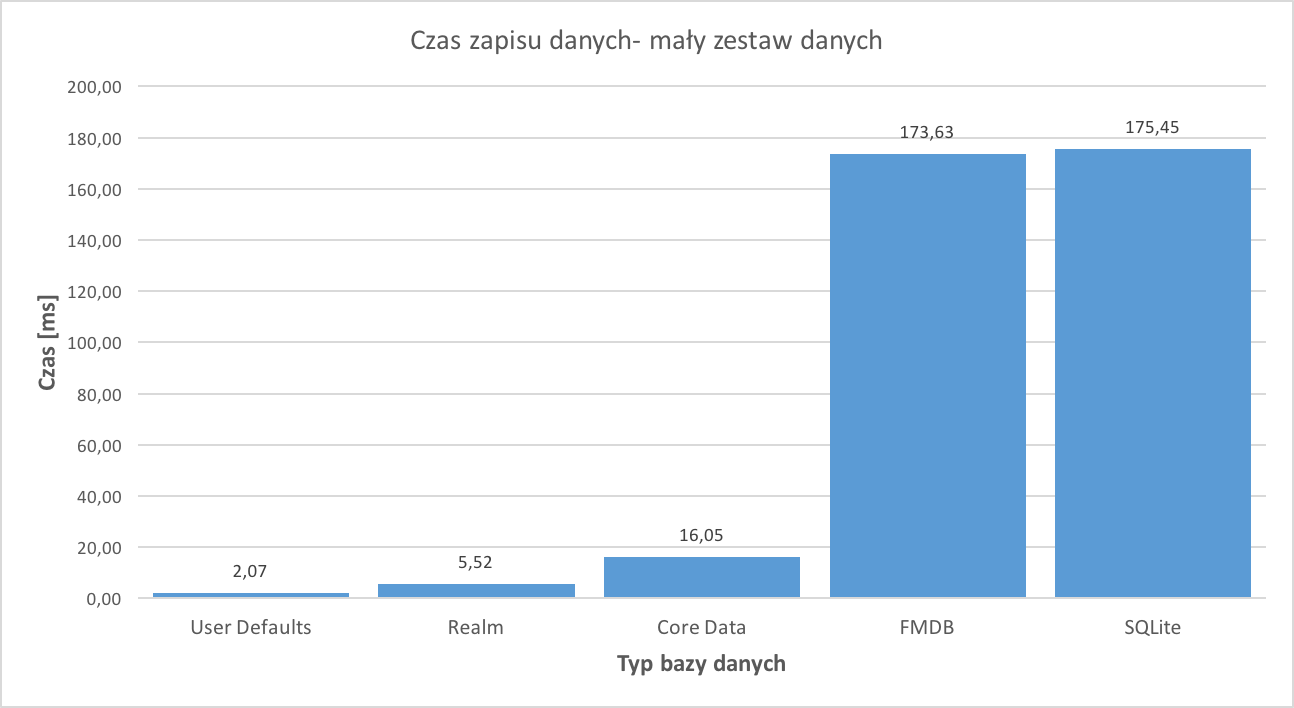
\includegraphics[width=15cm]{img/save_data/save_speed_small.png}
	\caption{Czasy zapisu danych do bazy - mały zestaw danych}
	\label{fig: small-save-time}
\end{figure}

\begin{figure}[h]
\centering
	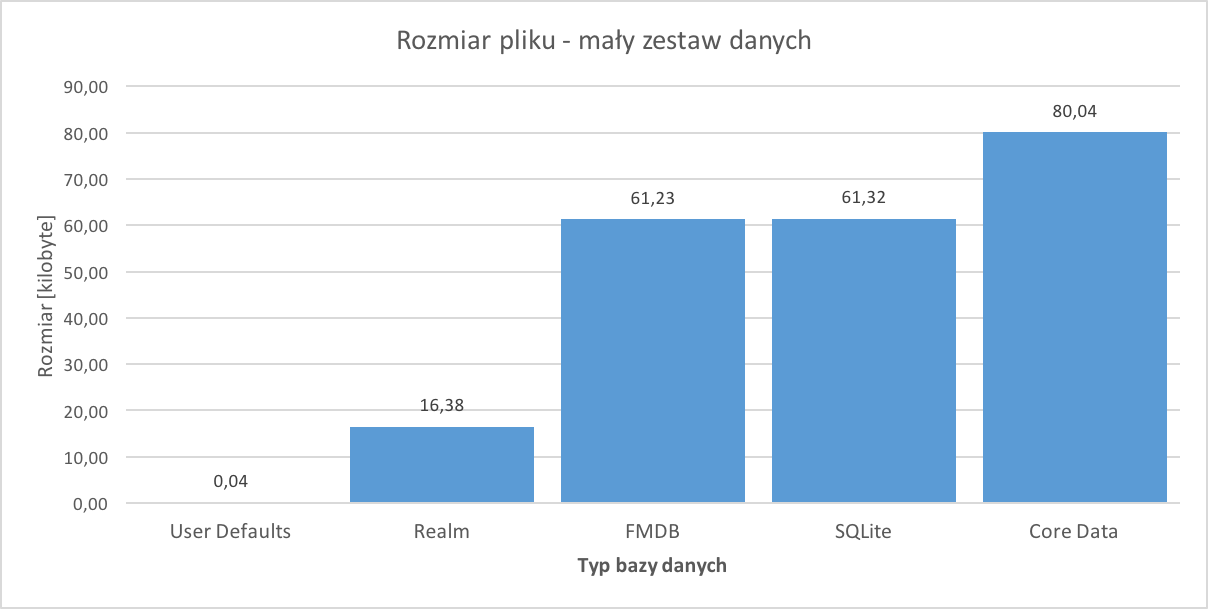
\includegraphics[width=15cm]{img/save_data/save_file_small.png}
	\caption{Rozmiar pliku wynikowego bazy danych - mały zestaw danych}
	\label{fig: small-save-file-size}
\end{figure}

\newpage

\begin{figure}[h]
\centering
	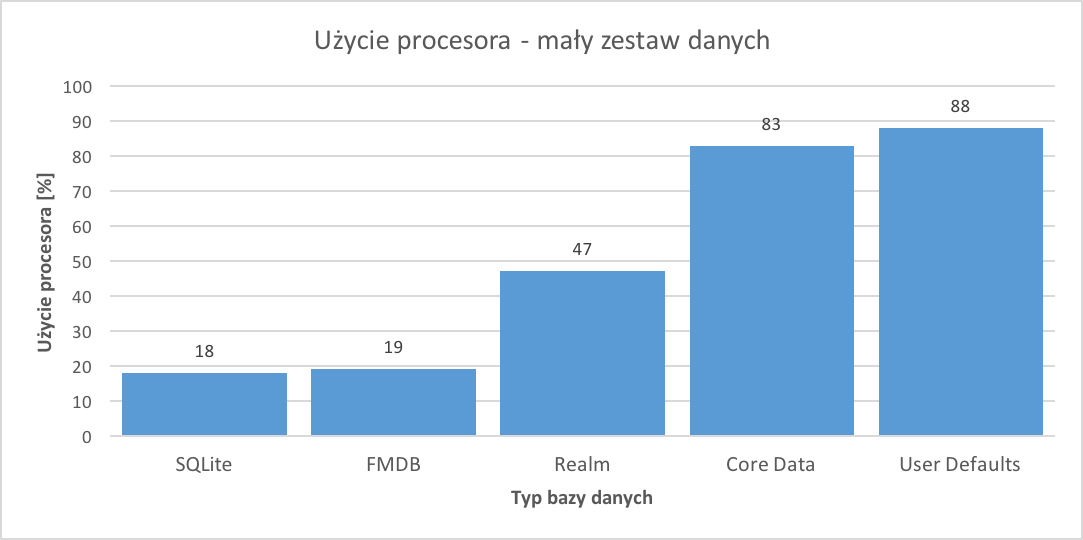
\includegraphics[width=15cm]{img/save_data/save_cpu_small.png}
	\caption{Użycie procesora podczas operacji - mały zestaw danych}
	\label{fig: small-save-cpu}
\end{figure}

\begin{figure}[h]
\centering
	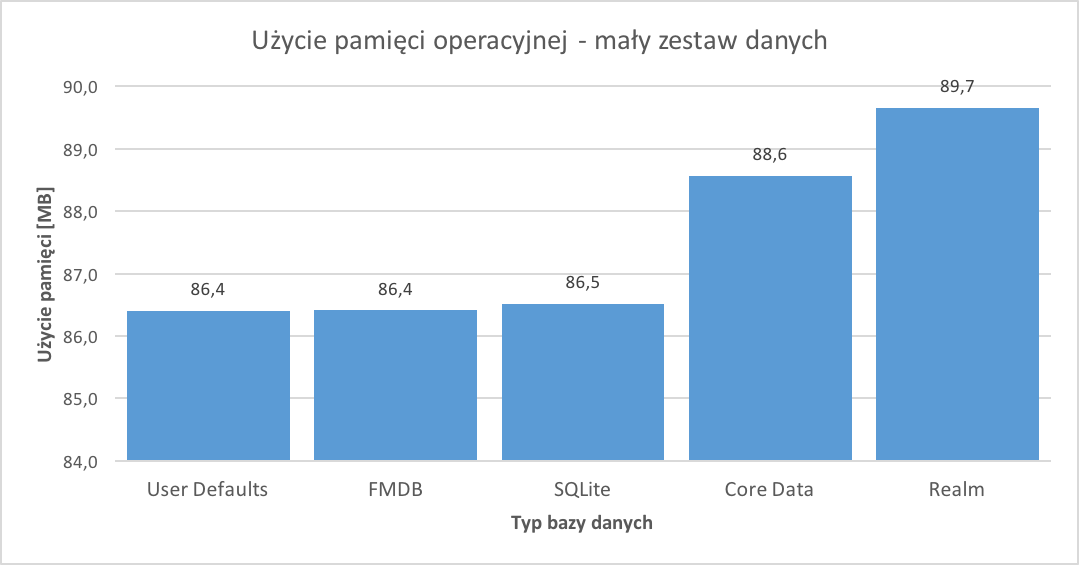
\includegraphics[width=15cm]{img/save_data/save_ram_small.png}
	\caption{Użycie pamięci operacyjnej podczas operacji - mały zestaw danych}
	\label{fig: small-save-ram}
\end{figure}

\newpage

Czasy zapisu danych widoczne na wykresie \ref{fig: small-save-time} i~w tabeli \ref{tab: small-save-time-table} pokazują że najszybszy okazała się Domyślna Baza Użytkownika, wynika to z~zasady jej działania. Zapisywane są w~niej listy obiektów, nie zachodzi potrzeba ustawiania relacji pomiędzy tabelami. Z~czasem ponad dwukrotnie wyższym wynoszącym 5,52 ms drugi w~kolejności jest Realm. Core Data uzyskała czas trzykrotnie wyższy niż Realm wynoszący 16.05 ms. Najwolniejsze okazały się bazy SQLite i~FMDB uzyskując zbliżone czasy 173,63 ms i~175,45 ms. \par 

Rozmiary plików baz widoczne na wykresie \ref{fig: small-save-file-size} i~w tabeli \ref{tab: small-save-file-size-table} pokazują, że Domyślna Baza Użytkownika posiada najmniejszy rozmiar wynoszący 0.04 kb, przechowuje dane binarne w~wysokim stopniu kompresji. Baza danych Realm posiada plik dużo większy, jego rozmiar wynosi 16,38 kb. SQLite i~FMDB uzyskały niemal równe rozmiary plików. Zaś plik wynikowy Core Data uzyskał rozmiar największy 80 kb. \par

Dane pokazujące użycie procesora podczas operacji zapisu widoczne w~tabeli \ref{tab: small-save-cpu-table} i~na wykresie \ref{fig: small-save-cpu} dowodzą, że SQLite i~FMDB używają jedynie 18-19\% zasobów procesora urządzenia. Realm uzyskuje wynik ponad 50\% wyższy wynoszący 47\%, zaś framework Core Data osiąga aż 83\%. Domyślna Baza Użytkownika mimo iż uzyskuje najlepszy czas zapisu podczas wykonywania operacji używa aż 88\% zasobów procesora co jest najgorszym wynikiem.\par 

Podczas testu przy użyciu najmniejszego zestawu danych użycie pamięci operacyjnej urządzenia jest zbliżone dla wszystkich baz danych. Rezultaty widoczne w~tabeli \ref{tab: small-save-ram-table} oscylują w~granicach od 86 mb do 89 mb. Przy tak małej ilości danych różnice te można przyjąć za mało istotne. Kolejne testy pokażą znaczne rozbieżności wykorzystania pamięci RAM pomiędzy testowanymi bazami.

\newpage

\subsubsection{Średni zestaw danych}

Prezentacja danych w~formie tabel: 

\begin{table}[h]
\centering
\caption{Czasy zapisu danych do bazy - średni zestaw danych}
\label{tab: medium-save-time-table}
\begin{tabular}{|c|c|}
\hline
Baza danych   & Czas zapisu [ms] \\ \hline
User Defaults & 4,48             \\ \hline
Realm         & 36,46            \\ \hline
Core Data     & 150,01           \\ \hline
FBDB          & 1872,36          \\ \hline
SQLite        & 1877,78          \\ \hline
\end{tabular}
\end{table}

\begin{table}[h]
\centering
\caption{Rozmiar pliku wynikowego bazy danych - średni zestaw danych}
\label{tab: medium-save-file-size-table}
\begin{tabular}{|c|c|}
\hline
Baza danych   & Rozmiar pliku bazy danych [kb] \\ \hline
User Defaults & 0,08                           \\ \hline
Realm         & 106,99                         \\ \hline
SQLite        & 318,34                         \\ \hline
FBDB          & 326,34                         \\ \hline
Core Data     & 592,94                         \\ \hline
\end{tabular}
\end{table}

\newpage

\begin{table}[h]
\centering
\caption{Użycie procesora podczas operacji - średni zestaw danych}
\label{tab: medium-save-cpu-table}
\begin{tabular}{|c|c|}
\hline
Baza danych   & Użycie procesora [\%] \\ \hline
SQLite        & 16                    \\ \hline
FMDB          & 19                    \\ \hline
Realm         & 77                    \\ \hline
User Defaults & 96                    \\ \hline
Core Data     & 97                    \\ \hline
\end{tabular}
\end{table}

\begin{table}[h]
\centering
\caption{Użycie pamięci operacyjnej podczas operacji - średni zestaw danych}
\label{tab: medium-save-ram-table}
\begin{tabular}{|c|c|}
\hline
Baza danych   & Użycie pamięci RAM [mb] \\ \hline
User Defaults & 91,3                    \\ \hline
FMDB          & 91,4                    \\ \hline
SQLite        & 91,4                    \\ \hline
Realm         & 94,8                    \\ \hline
Core Data     & 102,7                   \\ \hline
\end{tabular}
\end{table}

\newpage

Prezentacja wyników w~formie wykresów: 

\begin{figure}[h]
\centering
	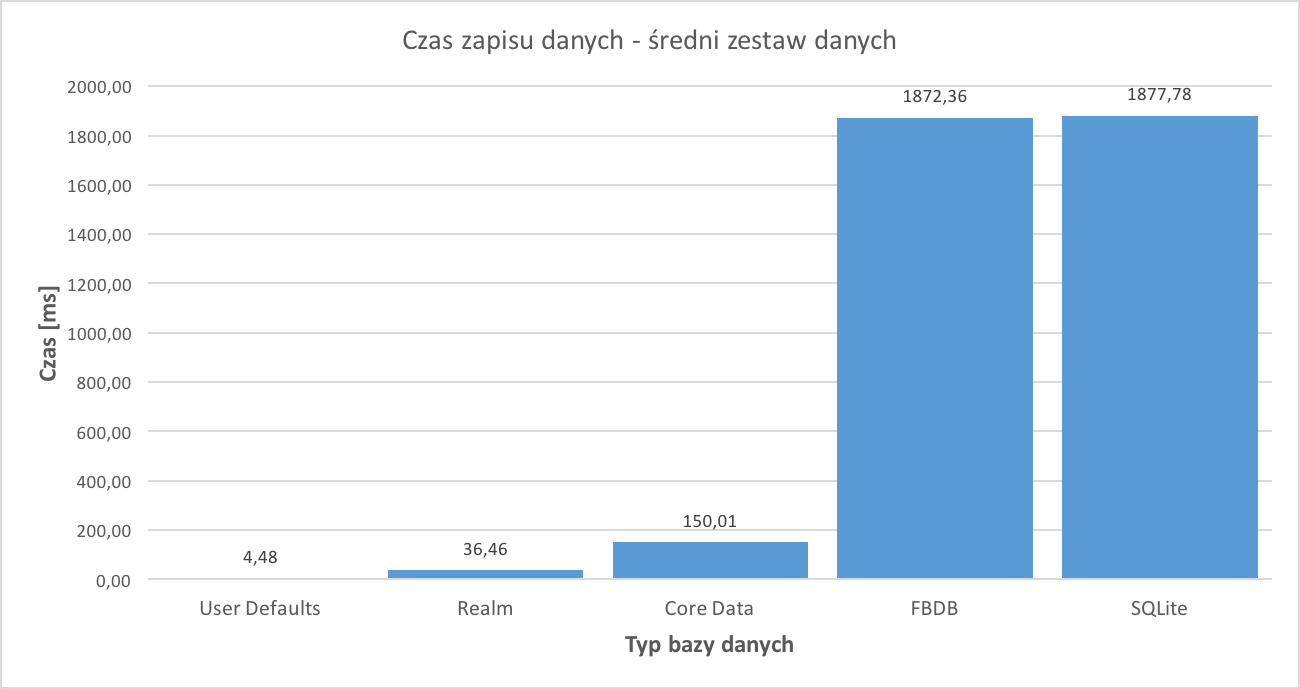
\includegraphics[width=15cm]{img/save_data/save_speed_medium.png}
	\caption{Czasy zapisu danych do bazy - średni zestaw danych}
	\label{fig: medium-save-time}
\end{figure}

\begin{figure}[h]
\centering
	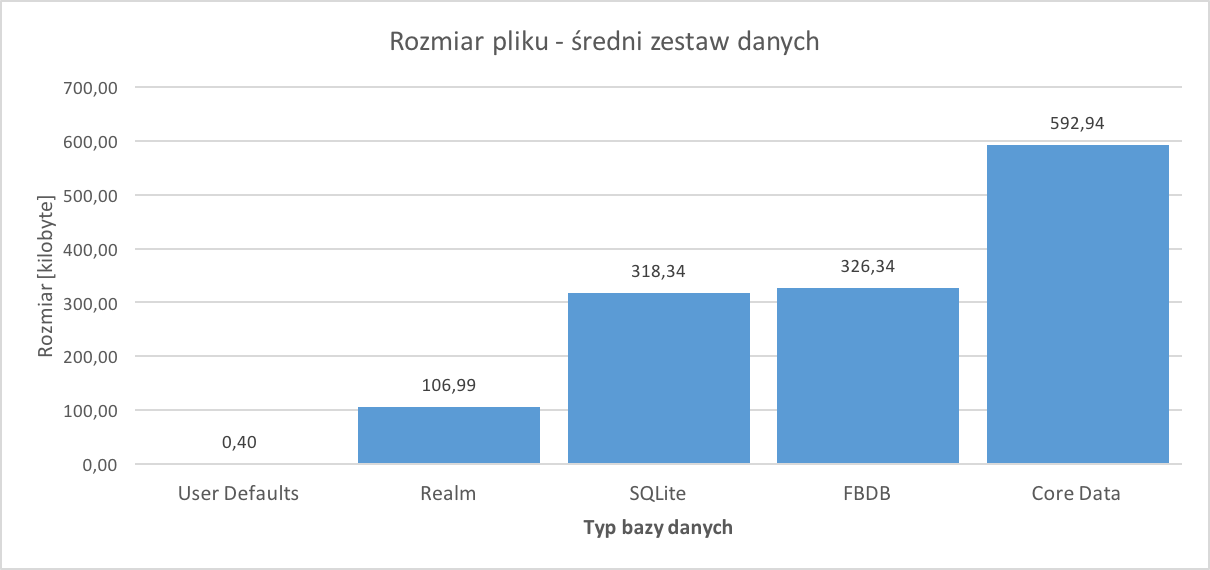
\includegraphics[width=15cm]{img/save_data/save_file_medium.png}
	\caption{Rozmiar pliku wynikowego bazy danych - średni zestaw danych}
	\label{fig: medium-save-file-size}
\end{figure}

\newpage

\begin{figure}[h]
\centering
	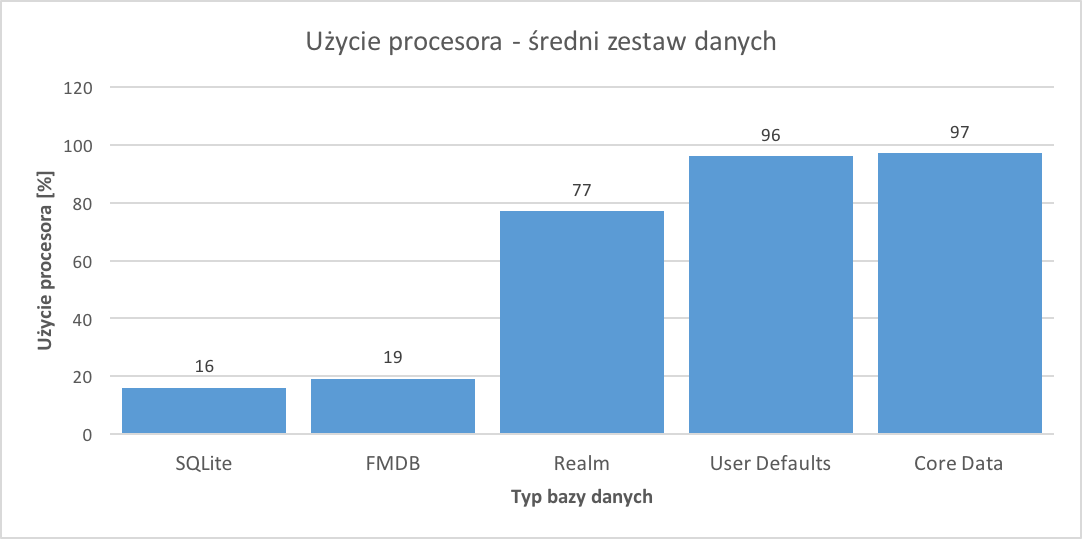
\includegraphics[width=15cm]{img/save_data/save_cpu_medium.png}
	\caption{Użycie procesora podczas operacji - średni zestaw danych}
	\label{fig: medium-save-cpu}
\end{figure}

\begin{figure}[h]
\centering
	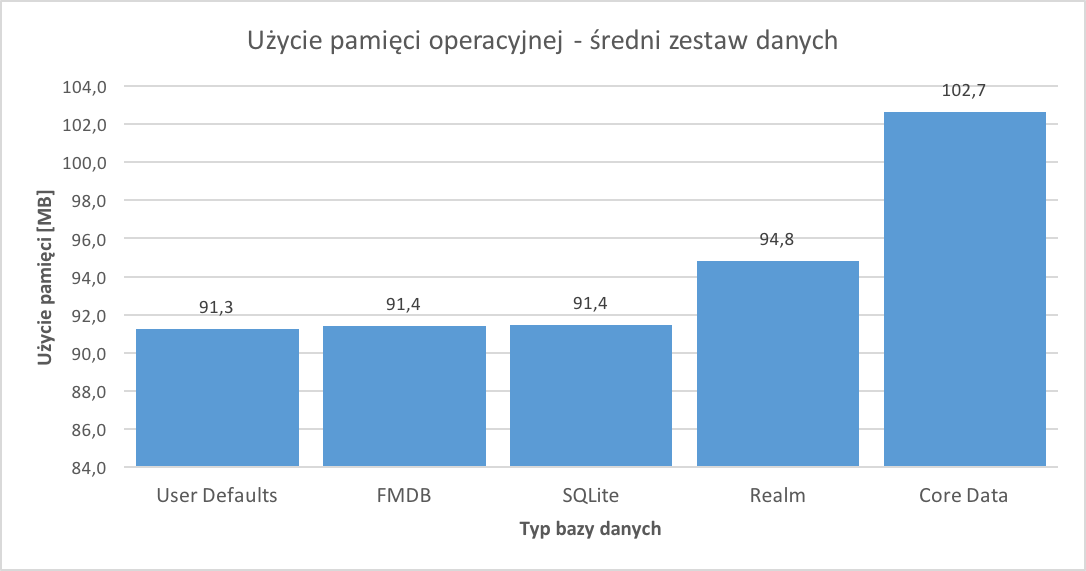
\includegraphics[width=15cm]{img/save_data/save_ram_medium.png}
	\caption{Użycie pamięci operacyjnej podczas operacji - średni zestaw danych}
	\label{fig: medium-save-ram}
\end{figure}

\newpage

Czasy zapisu danych podczas testu z~średnim zestawem danych  widoczne na wykresie \ref{fig: medium-save-time} pokazały tą samą klasyfikacje baz danych co test z~użyciem małego zestawu danych. Czas potrzebny na zapis danych wzrósł o~ponad 50\% dla Domyślnej Bazy Użytkownika, 80\% dla Realm, 85\% dla Core Data. SQLite i~FMDB potrzebowały ponad 90\% czasu więcej aby zapisać dane średniego zestawu. \par

Podobna sytuacja występuje przy wynikach wielkości plików wynikowych zaprezentowanych na wykresie \ref{fig: medium-save-file-size}. Klasyfikacja baz jest identyczna jak w~poprzednim teście. Plik Domyślnej Bazy Użytkownika osiągnął rozmiar o~90\% większy. Realm, SQLite, FMDB i~Core Data osiągnęły podobny przyrost pliku wynoszący 85\%. \par 

Użycie procesora podczas testu z~średnim zestawem danych widoczne na wykresie \ref{fig: medium-save-cpu} w~dalszym ciągu dowodzi, że pomimo wzrostu ilości danych SQLite i~FMDB zużywa najmniej zasobów procesora. W~przypadku Realm wykorzystanie CPU wzrosło o~40\%. Core Data i~Domyślna baza użytkownika przy większej ilości danych używały procesora w~96-97\%. \par 

Wykorzystanie pamięci operacyjnej dla SQLite, FMDB i~Domyślnej Bazy Użytkownika wzrosło o~5-6\% co pokazuje wykres \ref{fig: medium-save-ram}. Realm uzyskał lepszy rezultat względem poprzedniego testu zmniejszając wykorzystanie pamięci RAM o~5\%. Core Data wypadła najgorzej osiągając 103 MB. \par


\subsubsection{Duży zestaw danych}

Prezentacja danych w~formie tabel: 

\begin{table}[h]
\centering
\caption{Czasy zapisu danych do bazy - duży zestaw danych}
\label{tab: big-save-time-table}
\begin{tabular}{|c|c|}
\hline
Baza danych   & Czas zapisu [ms] \\ \hline
User Defaults & 30,48            \\ \hline
Realm         & 201,93           \\ \hline
Core Data     & 24912,73         \\ \hline
FMDB          & 34217,17         \\ \hline
SQLite        & 35044,62         \\ \hline
\end{tabular}
\end{table}

\newpage

\begin{table}[h]
\centering
\caption{Rozmiar pliku wynikowego bazy danych - duży zestaw danych}
\label{tab: big-save-file-size-table}
\begin{tabular}{|c|c|}
\hline
Baza danych   & Rozmiar pliku bazy danych [kb] \\ \hline
User Defaults & 4,00                           \\ \hline
Realm         & 2588,67                        \\ \hline
SQLite        & 3177,88                        \\ \hline
FMDB          & 3264,30                        \\ \hline
Core Data     & 7240,79                        \\ \hline
\end{tabular}
\end{table}

\begin{table}[h]
\centering
\caption{Użycie procesora podczas operacji - duży zestaw danych}
\label{tab: big-save-cpu-table}
\begin{tabular}{|c|c|}
\hline
Baza danych   & Użycie procesora [\%] \\ \hline
SQLite        & 16                    \\ \hline
FMDB          & 19                    \\ \hline
Realm         & 88                    \\ \hline
Core Data & 98                    \\ \hline
User Defaults    & 97                    \\ \hline
\end{tabular}
\end{table}

\begin{table}[h]
\centering
\caption{Użycie pamięci operacyjnej podczas operacji - duży zestaw danych}
\label{tab: big-save-ram-table}
\begin{tabular}{|c|c|}
\hline
Baza danych   & Użycie pamięci RAM [mb] \\ \hline
SQLite        & 133,2                   \\ \hline
FMDB          & 134,9                   \\ \hline
Realm         & 141,6                   \\ \hline
User Defaults & 145,7                   \\ \hline
Core Data     & 258,5                   \\ \hline
\end{tabular}
\end{table}

\newpage

Prezentacja wyników w~formie wykresów: 

\begin{figure}[H]
\centering
	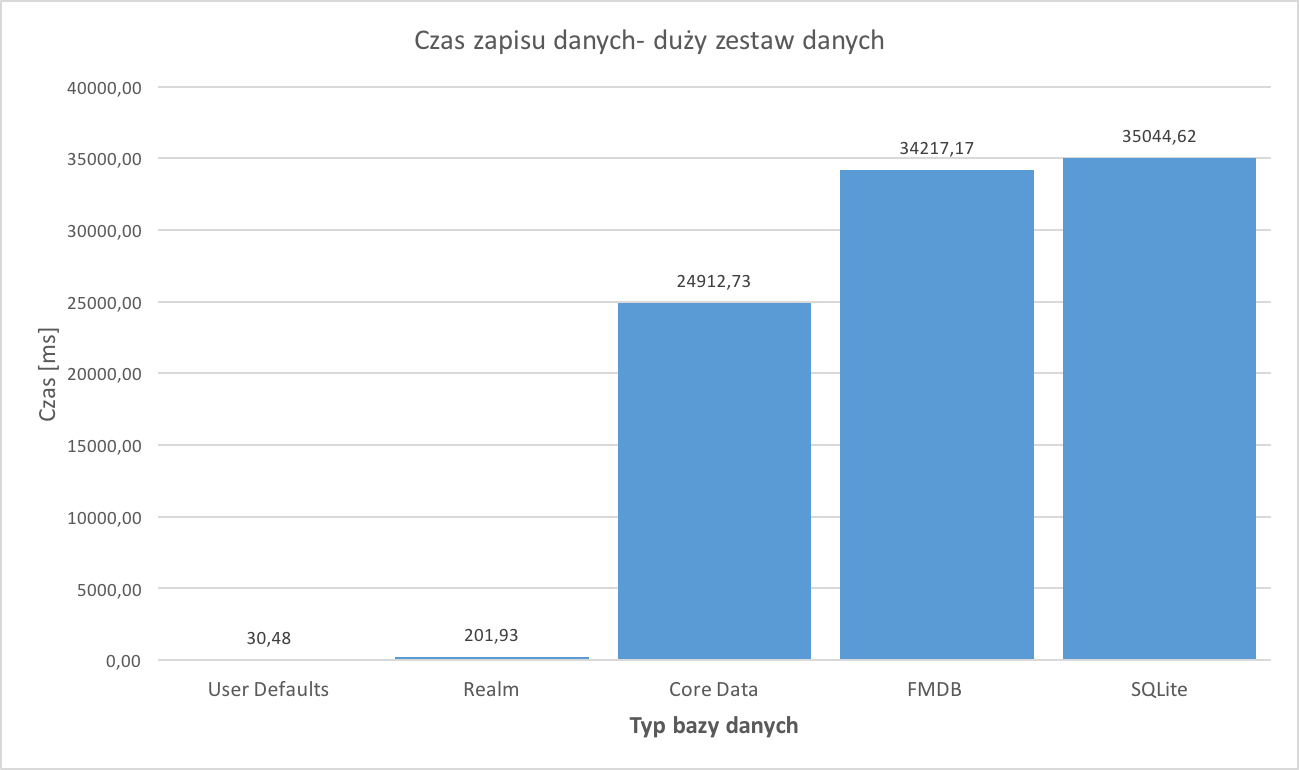
\includegraphics[width=13.5cm]{img/save_data/save_speed_big.png}
	\caption{Czasy zapisu danych do bazy - duży zestaw danych}
	\label{fig: big-save-time}
\end{figure}

\begin{figure}[H]
\centering
	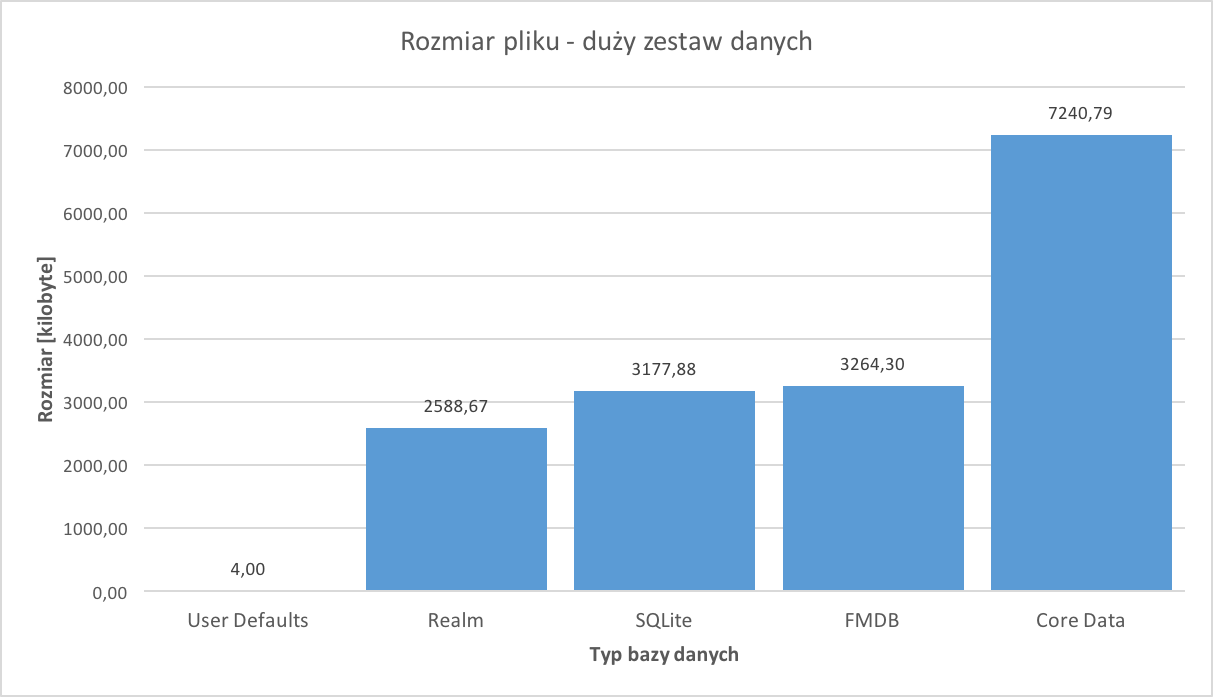
\includegraphics[width=13.5cm]{img/save_data/save_file_big.png}
	\caption{Rozmiar pliku wynikowego bazy danych - duży zestaw danych}
	\label{fig: big-save-file-size}
\end{figure}

\begin{figure}[H]
\centering
	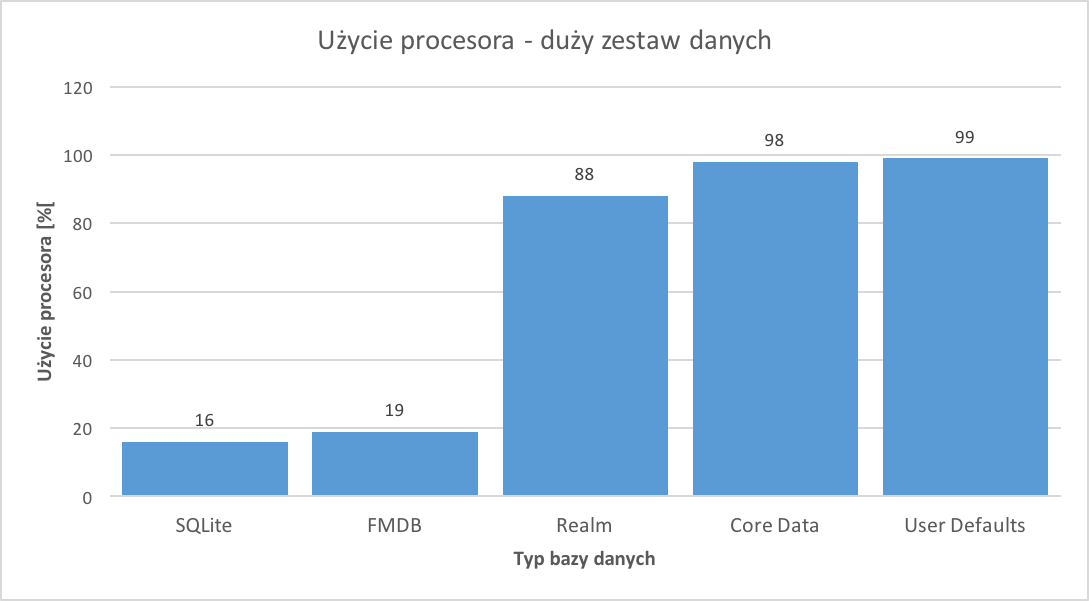
\includegraphics[width=15cm]{img/save_data/save_cpu_big.png}
	\caption{Użycie procesora podczas operacji - duży zestaw danych}
	\label{fig: big-save-cpu}
\end{figure}

\begin{figure}[H]
\centering
	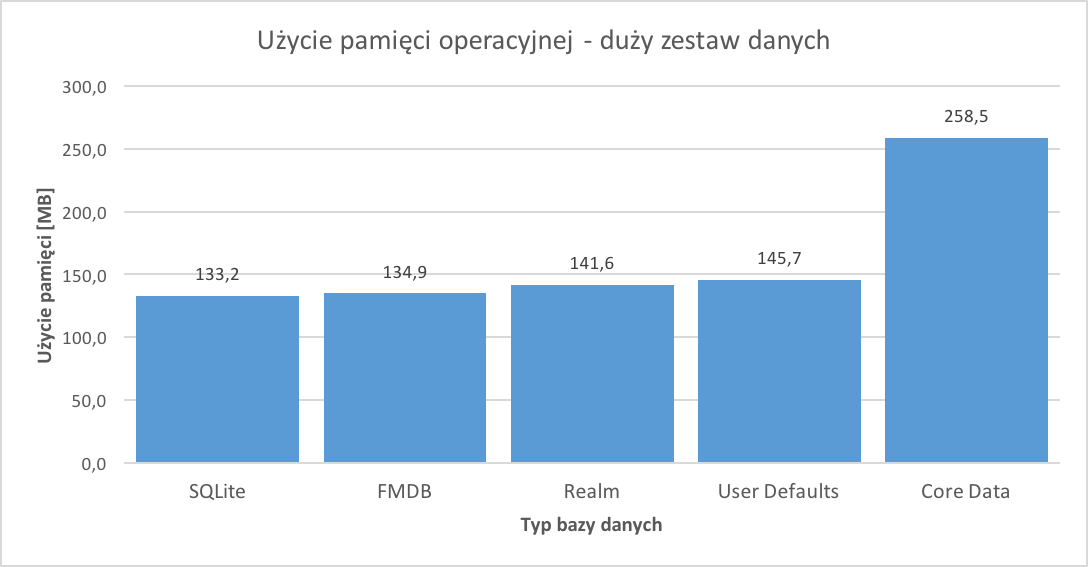
\includegraphics[width=15cm]{img/save_data/save_ram_big.png}
	\caption{Użycie pamięci operacyjnej podczas operacji - duży zestaw danych}
	\label{fig: big-save-ram}
\end{figure}

\newpage

Czasy zapisu danych pokazane na wykresie \ref{fig: big-save-time} udowadniają, że wraz ze wzrostem ilości danych Domyślna Baza Użytkownika i~Realm mają stały przyrost czasu względem dwóch poprzednich testów wynoszący około 85\%. Sytuacja zmienia się w~przypadku pozostałych baz danych. Core Data w~teście z~największym zestawem danych wypada o~wiele gorzej niż w~poprzednich testach. Czas zapisu danych sięga tu 25 sekund. Gorzej względem poprzednich testów wypada SQLite i~FMDB osiągając czasy 34-35 sekund. 

Rozmiary plików wynikowych w~teście z~największą ilością danych widoczny na wykresie \ref{fig: big-save-file-size} pokazują, że Domyślna Baza Użytkownika zwiększa rozmiar wykładniczo względem poprzednich testów. Plik bazy Realm osiąga rozmiar 2588 kb jest to 25\% więcej niż w~teście ze średnim zestawem danych. FMDB i~SQLite zwiększyły swój rozmiar pliku o~10\% zaś Core Data zwiększyła rozmiar pliku o~12%. 

Użycie procesora podczas testu z~wielkim zestawem danych pokazane na wykresie \ref{fig: big-save-cpu} pokazuje, że w~dalszym ciągu SQLite i~FMDB nie zwiększają zapotrzebowania na moc obliczeniową. Realm w~tym teście potrzebował 10\% wykorzystania procesora, zaś Domyślna Baza Użytkownika i~Core Data pokazały największe zapotrzebowanie wynoszące 98-99\%. 

 W~przypadku użycia pamięci RAM widocznego na wykresie \ref{fig: big-save-ram} można zauważyć, że SQLite i~FMDB posiadają najmniejsze wartości wynoszące 133-135 MB. Realm zachowuje zbliżony rezultat wynoszący 141 MB. Zapotrzebowanie zwiększyła Domyślna Baza Użytkownika zajmując przedostatnie miejsce z~wartością 145 MB. Core Data zaś potrzebowała aż 258 MB pamięci operacyjnej do operacji zapisu największego zestawu danych, jest to 150\% więcej niż w~poprzednim teście. 

\subsubsection{Podsumowanie - zapis danych}

 Z~testów wynika, że najszybszy zapis danych możliwy jest przy wykorzystaniu Domyślnej Bazy Użytkownika. Realm posiada we wszystkich testach drugi rezultat. Core Data świetnie radzi sobie przy zapisie małej i~średniej ilości danych, natomiast czas zapisu drastycznie rośnie w~przypadku wielkiej liczby danych. SQLite i~FMDB osiągają najgorsze rezultaty, wynikać to może z~surowej implementacji obsługi konwersji danych podczas zapisu. 

 W~wielkości pliku wynikowego także dominuje Domyślna Baza Użytkownika a~zaraz po niej jest Realm. SQLite i~FMDB posiadają pliki niemal tej samej wielkości. Core Data ze względu na zapis do swojego pliku nie tylko samych danych a~także danych przechowujących graficzną reprezentacje bazy oraz wszelkich konfiguracji wykorzystywanych przed środowisko programistyczne XCode osiąga wielkie rozmiary plików wynikowych. 

Najmniejsze zużycie procesora wykazują bazy SQLite i~FMDB. W~przypadku Realm wykorzystanie mocy CPU zależne jest od ilości przetwarzanych danych i~rośnie wraz z~ich ilością. Core Data i~Domyślna Baza Użytkownika wymagają najwięcej zasobów procesora do przeprowadzenia operacji zapisywania danych. 

Wraz ze wzrostem ilości danych rośnie też zapotrzebowanie na pamięć operacyjna urządzenia. W~przypadku małej ilości danych wszystkie bazy wykazują niewielkie zapotrzebowanie na pamięć RAM. Największe różnice widoczne są przy wielkiej ilości danych. Najlepiej w~tej sytuacji radzą sobie bazy SQL, drugie miejsce zajmuje Realm. Core Data wymaga największej  ilości pamięci operacyjnej. 

\subsection{Testy odczytu danych}

Podrozdział przedstawia testy odczytu danych w~kliku różnych scenariuszach: 

\begin{itemize}
\item Odczyt wszystkich danych z~tabel.
\item Wyszukanie wszystkich autorów o~imieniu "Diena".
\item Wyszukanie 2 książek z~największa liczbą autorów.
\item Odczyt maksymalnie 20 wydawnictw z~największą liczba wydanych książek i~posortowanie wyniku rosnąco.
\end{itemize}

Zastosowanie różnych operacji odczytywania danych ma na celu sprawdzenie jak testowane bazy danych radzą sobie podczas wykonywania zapytań. Wykonanie jedynie jednej operacji nie pozwoliło by uzyskać zadowalających rezultatów gdyż wiadomo iż każda z~baz danych inaczej będzie wykonywać każdą z~przeprowadzanych operacji. Tak samo jak w~przypadku testowania zapisu danych każda z~operacji zostały przeprowadzone na trzech różnych zestawach danych oraz każdy z~testów wykonany został sto razy a~prezentowany wynik jest średnią z~wszystkich stu operacji. 

\newpage

\subsubsection{Odczyt wszystkich danych}

\begin{figure}[h]
\centering
	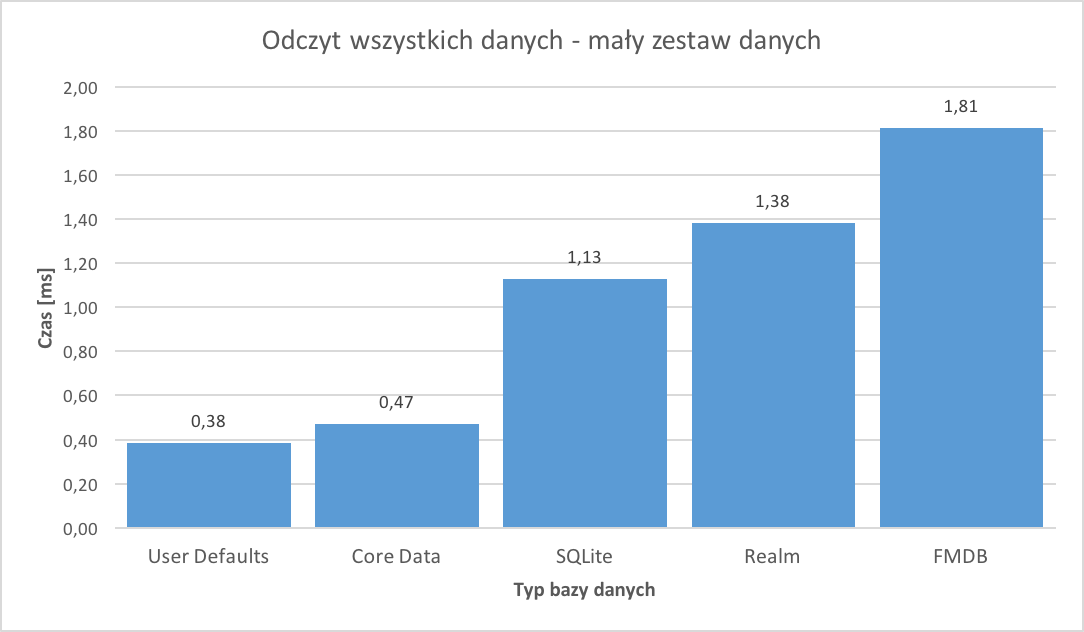
\includegraphics[width=13.5cm]{img/read_data/read_all/read_all_test_small.png}
	\caption{Czas odczytu wszystkich danych - mały zestaw danych}
	\label{fig: read-data-small}
\end{figure}

\begin{figure}[h]
\centering
	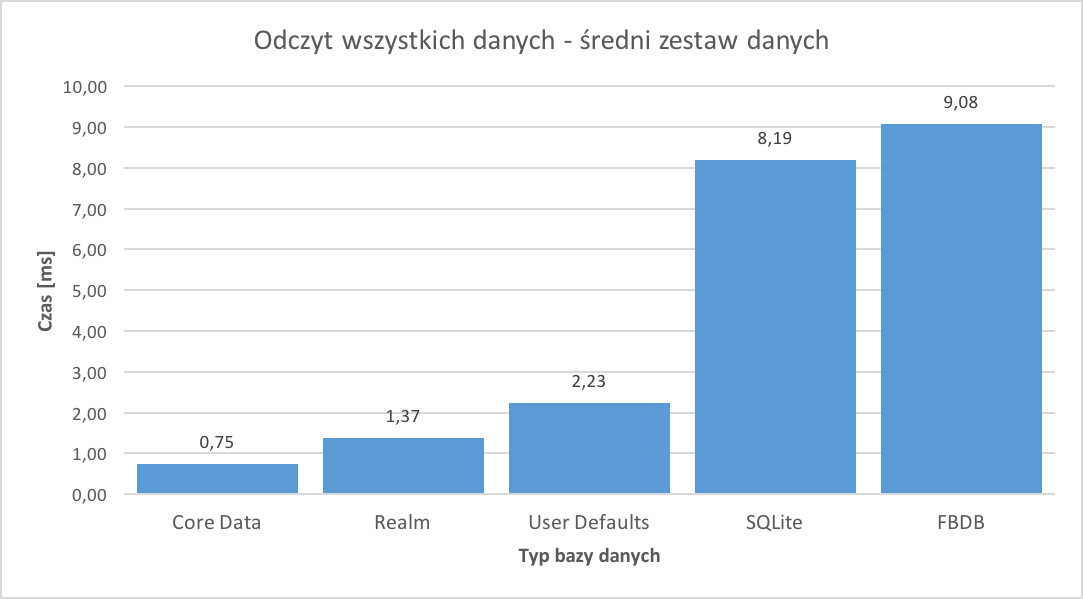
\includegraphics[width=13.5cm]{img/read_data/read_all/read_all_test_medium.png}
	\caption{Czas odczytu wszystkich danych - średni zestaw danych}
	\label{fig: read-data-medium}
\end{figure}

\newpage

\begin{figure}[h]
\centering
	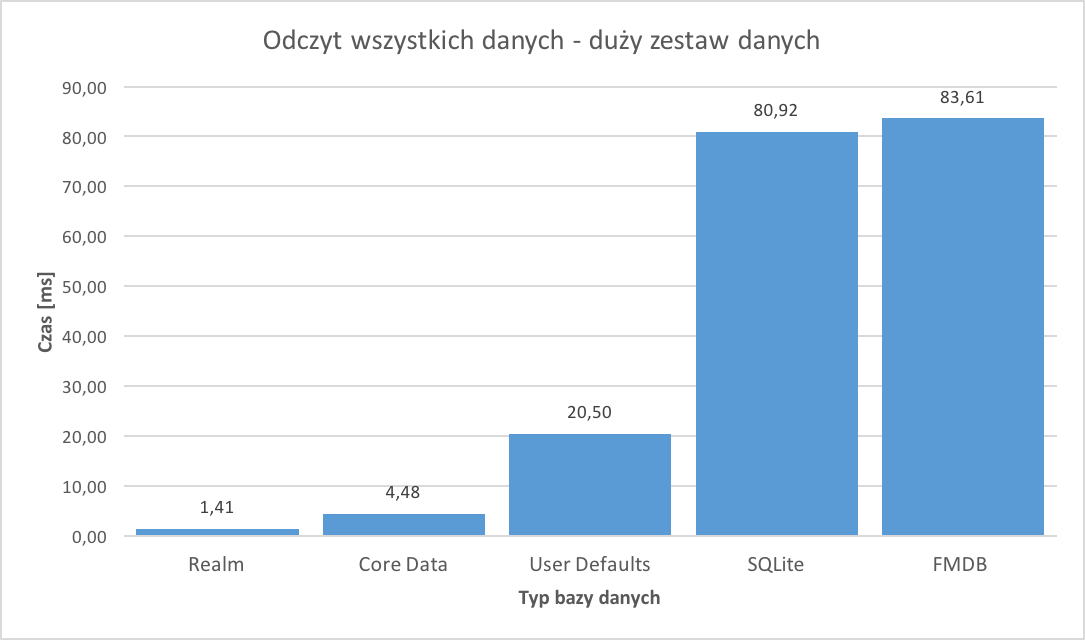
\includegraphics[width=15cm]{img/read_data/read_all/read_all_test_big.png}
	\caption{Czas odczytu wszystkich danych - duży zestaw danych}
	\label{fig: read-data-big}
\end{figure}

Rezultaty odczytu wszystkich danych z~baz prezentują różne wyniki zależne od ilości danych. W~przypadku małego zestawu danych najmniejszy czas równy 0.38 ms uzyskała Domyślna Baza Użytkownika. Zaraz po niej z~czasem 0.47 ms znajduje się Core Data. SQLite uzyskał czas 1.13 ms. Baza danych Realm odczytała wszystkie dane w~czasie 1.38 ms. Najwolniejsza okazała się FMDB dając rezultat 1.81 ms. 

 W~przypadku odczytu średniego zestawu danych najszybsza okazała się Core Data uzyskując czas 0.75 ms. Realm zaś odczytał dane zestawu średniego w~czasie 1.37 ms, czas ten różnie się zaledwie o~0.01 ms od wyniku uzyskanego przez tą bazę danych przy odczycie małego zestawu danych. Domyślna Baza Użytkownika uzyskała czas 2.23 ms co jest rezultatem gorszym aż o~1.85 względem testu z~użyciem małego zestawu danych. Najwolniejsze okazały się SQLite z~czasem 8,19 ms i~FMDB z~czase 9.08 ms. 

Testy z~użyciem dużego zestawu danych pokazują, że Realm jest najszybszą bazą danych jeżeli chodzi o~odczyt wszystkich danych znajdujących się w~bazie. Czas odczytu największej ilości danych to zaledwie 1.41 ms. Core Data uzyskała drugi rezultat z~czasem 4.48 ms. Domyślna Baza Użytkownika odczytała dane w~czasie 20.50 ms. SQLite i~FMDB odczytały dane w~najdłuższym czasie wynoszącym ponad 80 ms. 

Można więc zaważyć, że Realm mimo słabych rezultatów w~testach z~małym i~średnim zestawem danych uzyskał doskonały rezultat podczas największego testu. Różnice w~czasach odczytu w~zależności od ilości danych przy użyciu Realm są bardzo niewielkie, wahają się w~granicach 0.04 ms. Domyślna Baza Użytkownika znacząco zwiększa czas odczytu danych wraz ze wzrostem ilości zapisanych danych. Czas odczytu danych w~przypadku użycia Core Data wzrasta wraz ze wzrostem ilości danych lecz przyrost czasu jest nie  duży względem reszty testowanych baz danych. Najwolniejsze i~z największym przyrostem czasowym okazały się bazy SQLite i~FMDB. 

\subsubsection{Wyszukanie wszystkich autorów o~imieniu ''Diena,,}

\begin{figure}[H]
\centering
	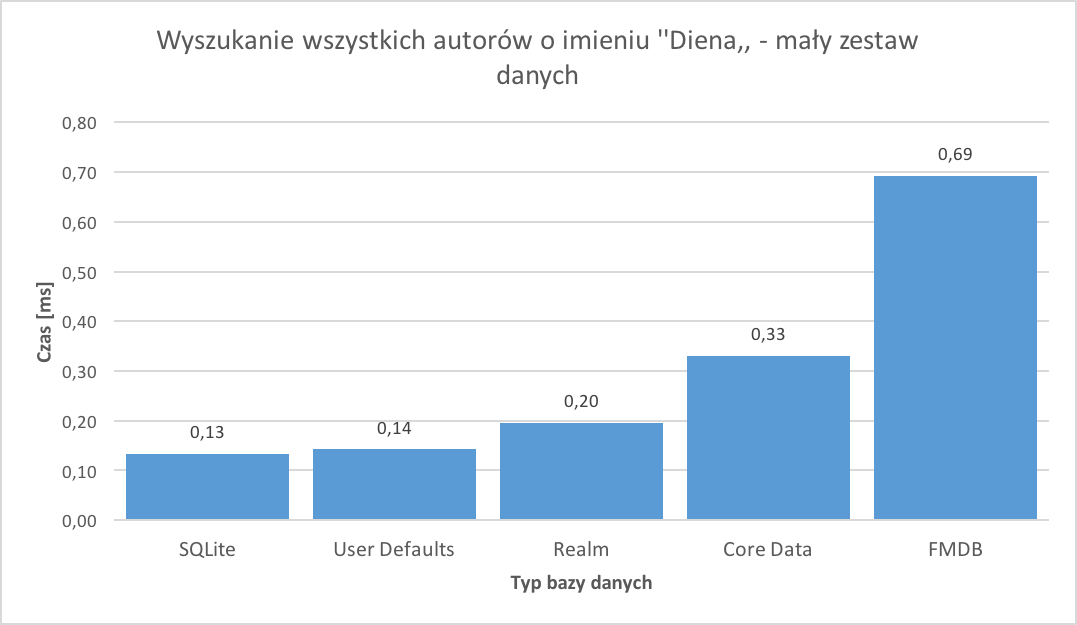
\includegraphics[width=15cm]{img/read_data/read_by_authors/read_by_author_small_test.png}
	\caption{Wyszukanie wszystkich autorów o~imieniu ''Diena,, - mały zestaw danych}
	\label{fig: read-by-author-small}
\end{figure}

\begin{figure}[H]
\centering
	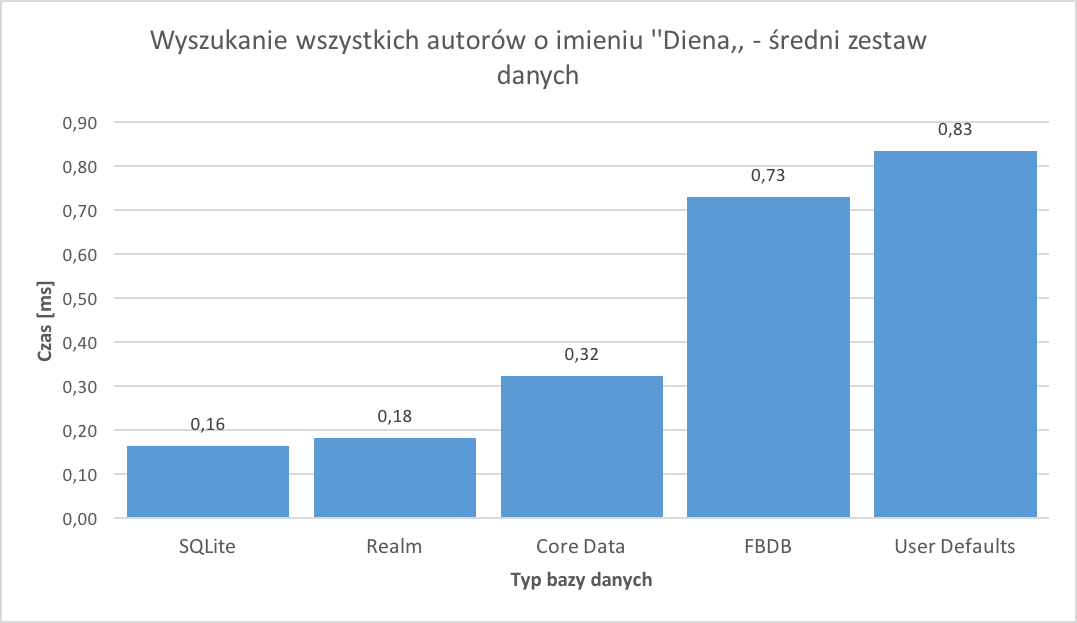
\includegraphics[width=15cm]{img/read_data/read_by_authors/read_by_author_medium_test.png}
	\caption{Wyszukanie wszystkich autorów o~imieniu ''Diena,, - średni zestaw danych}
	\label{fig: read-by-author-medium}
\end{figure}

\begin{figure}[H]
\centering
	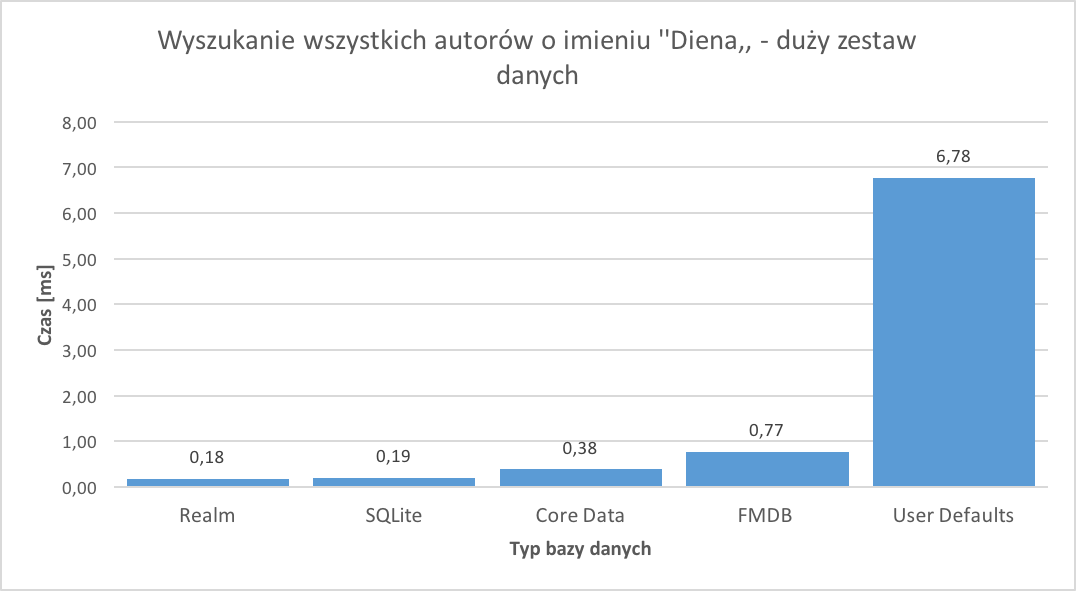
\includegraphics[width=15cm]{img/read_data/read_by_authors/read_by_author_big_test.png}
	\caption{Wyszukanie wszystkich autorów o~imieniu ''Diena,, - duży zestaw danych}
	\label{fig: read-by-author-big}
\end{figure}

Test odczytu autorów o~imieniu ''Diena,, przedstawia następujące wyniki. W~przypadku małego zestawu danych okazał się SQLite z~wynikiem 0.13 ms, na drugim miejscu znalazła się Domyślna Baza Użytkownika uzyskując czas 0.14 ms. Rezultat Realm widoczny na wykresie 6.16 wynosi 0.20 ms, baza ta jest więc wolniejsza o~0.07 ms od najszybszej SQLite. Core Data wyszukała dane w~czasie 0.33 ms. Dobrze widoczna jest różnica w~czasie FMDB od czystej bazy SQLite. Wraper odczytał dane w~czasie 0.69 ms, jest to rezultat gorszy o~0.56 ms od SQLite. 

Odczyt w~przypadku średniego zestawu danych pokazuję, że dziesięciokrotnie większa ilość rekordów względem poprzedniego testu  nie wpływa znacząco na bazy Realm, SQLite, Core Data i~FMDB. Rezultaty widoczne na wykresie \ref{fig: read-by-author-medium} są większe o~0.02 - 0.04 ms. Znaczącą różnice pokazuję zaś Domyślna Baza Użytkownika, odczytała ona dane w~czasie 0.83 ms co jest rezultatem o~85\% gorszym niż w~poprzednim teście. 

Także odczyt dużego zestawu danych nie wpłyną znacząco na uzyskane czasy otrzymania rezultatów. Na wykresie \ref{fig: read-by-author-big} widać, że tak jak poprzednio czasy dla baz Realm, SQLite, Core Data i~FMDB są większe o~0.02 - 0.04 ms w~porównaniu to poprzedniego testu. Domyślna Baza Użytkownika tak samo zwiększyła swój czas odczytu do 6.78 ms i~jest to rezultat także o~85\% większy niż w~poprzednim teście. 

Przedstawiona operacja odczytu autorów o~wybranym imieniu nie wymagała przetwarzania relacji w~bazach. Można tutaj zauważyć, które z~baz danych dobrze radzą sobie z~prostym przeszukiwaniem zapisanych danych. Realm i~SQLite przetwarzając różne ilości danych potrzebują bardzo zbliżonego czasu na znalezienie rezultatu zapytania. Core Data pomimo, iż jest blisko dwukrotnie wolniejsza od Realm i~SQLite także nie zwiększa znacząco czasu odczytu względem ilości danych. FMDB mimo iż jest wraperem SQLite okazuje się jednym z~najwolniejszych rozwiązań. Domyślna Baza Użytkownika radzi sobie znakomicie z~małą ilością danych. Wraz ze wzrostem liczby rekordów czas rośnie o~85\% przy zwiększaniu ilości danych dziesięciokrotnie.

\subsubsection{Wyszukanie 2 książek z~największa liczbą autorów}

\begin{figure}[H]
\centering
	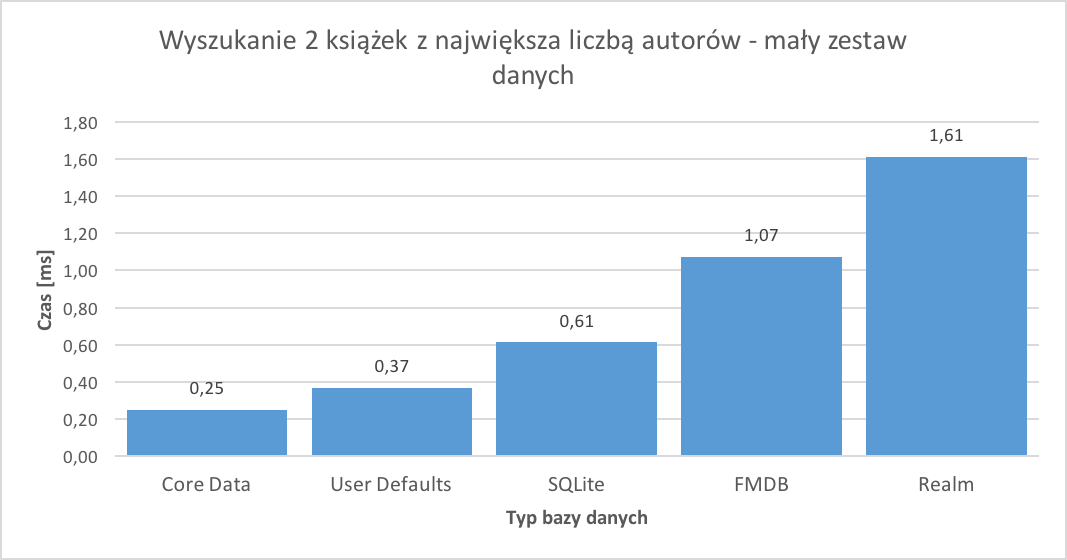
\includegraphics[width=15cm]{img/read_data/read_by_books/read_by_books_small_test.png}
	\caption{Wyszukanie 2 książek z~największa liczbą autorów - mały zestaw danych}
	\label{fig: read-by-books-small}
\end{figure}

\begin{figure}[H]
\centering
	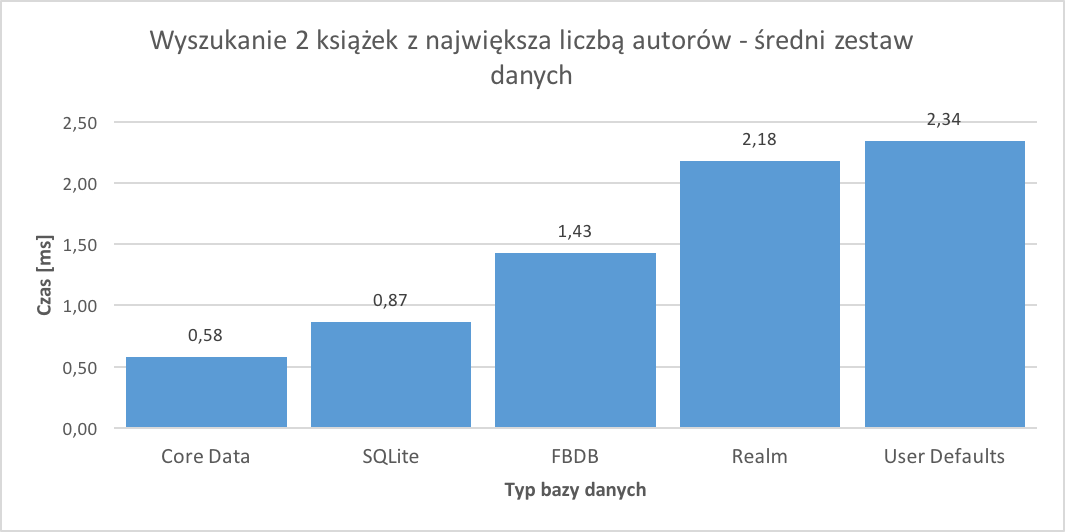
\includegraphics[width=15cm]{img/read_data/read_by_books/read_by_books_medium_test.png}
	\caption{Wyszukanie 2 książek z~największa liczbą autorów - średni zestaw danych}
	\label{fig: read-by-books-medium}
\end{figure}

\begin{figure}[H]
\centering
	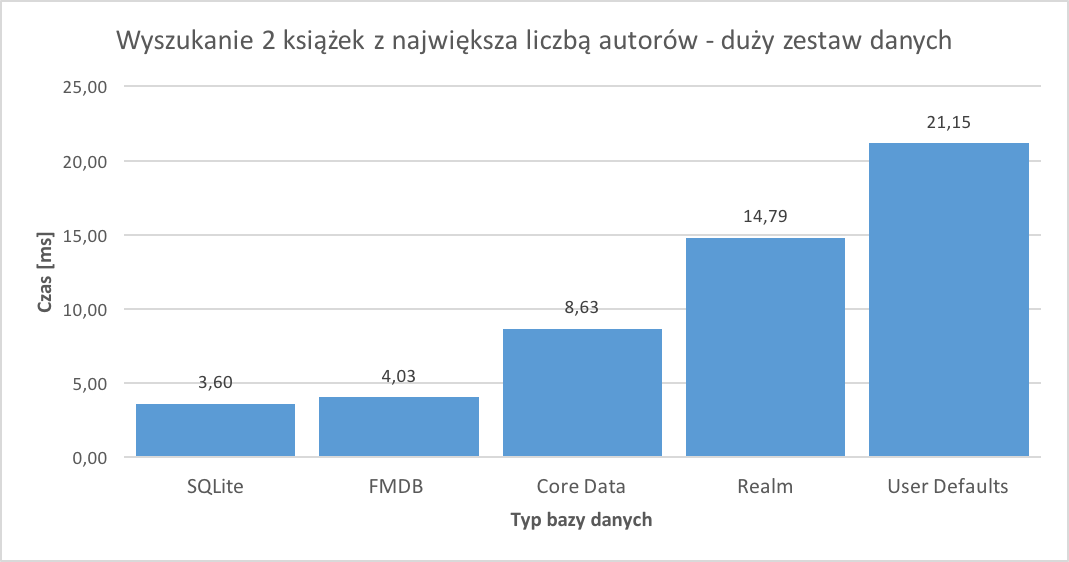
\includegraphics[width=15cm]{img/read_data/read_by_books/read_by_books_big_test.png}
	\caption{Wyszukanie 2 książek z~największa liczbą autorów - duży zestaw danych}
	\label{fig: read-by-books-big}
\end{figure}

Test wyszukania książek z~największą liczbą autorów wymagał wspierania się relacjami pomiędzy tabelami książka i~autor. Wyniki testów pokazują znaczące różnice w~szybkości działania baz w~porównaniu do testu przeszukiwania jednej tabeli. 

Wykres \ref{fig: read-by-books-small} przedstawia rezultaty wyszukanie 2 książek z~największa liczbą autorów w~przypadku użycia małego zestawu danych. Najszybsza okazała się Core Data uzyskując czas równy 0.25 ms. Z~małą ilością danych dobrze poradziła sobie też Domyślna Baza Użytkownika uzyskując rezultat 0.37 ms. Trzeci w~kolejności jest SQLite z~czasem 0.61 ms. Ponownie wolniejszy od SQLite okazał się FMDB, zwrócił on rezultat w~czasie 1.07 ms. Najwolniejsza jest baza Realm, uzyskała ona czas 1.61 ms.

Dane przedstawione na wykresie \ref{fig: read-by-books-medium} pokazują rezultatu testu z~użyciem średniego zestawu danych. Core Data uzyskała najmniejszy czas 0.58 ms jest to rezultat o~55\% większy od testu z~małym zestawem danych. SQLite zakończył zadanie w~czasie 0.87 ms, zaś FMDB ponownie okazał się wolniejszy od SQLite uzyskując czas 1.43 ms. Przedostatni rezultat uzyskał Realm, czas operacji wyniósł 2.18 ms. Domyślna Baza Użytkownika po raz kolejny podczas zwiększenia ilości danych uzyskuję znacznie gorsze wyniki. Baza zwróciła rezultat w~czasie 2.34 ms i~kolejny raz jest to rezultat większy o~85\% od testu na małym zestawie danych. 

Test z~użyciem dużego zestawu danych, którego wyniki widoczne są na wykresie \ref{fig: read-by-books-big} pokazuje przewagę SQL-a w~operacjach na dużej liczbie danych. Najszybsze okazują się tu bazy SQLite i~FMDB. SQLite uzyskał czas 3.60 ms zaś FMDB 4.03 ms. Trzeci rezultat uzyskała Core Data, potrzebowała ona 90\% czasu więcej niż w~teście poprzednim lecz w~dalszym ciągu ukończyła zadanie z~dobrym czasem wynoszącym 8.63 ms. Jedną z~najwolniejszych baz okazał się Realm, zrealizował on zapytanie w~czasie 14.79 ms. Najwolniejsza okazała się ponownie Domyślna Baza Użytkownika uzyskując czas 21.15 ms. 

Powyższy test pokazuję przewagę rozwiązań SQL w~bardziej skomplikowanych operacjach niż przeszukanie jednej tabeli. Rozwiązania takie jak SQLite i~FMDB okazują się wolniejsze w~przypadku małej i~średniej liczby danych lecz zyskują wiele w~przypadku dużej ilości danych. Core Data uzyskuję czasy coraz większe wraz z~liczbą rekordów lecz nie jest to tak znacząca różnica jak w~przypadku Realm czy Domyślnej Bazy Użytkownika, która okazała się najwolniejsza w~przedstawionym teście niezależnie od zestawu danych. 

\subsubsection{Odczyt maksymalnie 20 wydawnictw z~największą liczba wydanych książek oraz posrotowanie wyniku rosnąco}

\begin{figure}[H]
\centering
	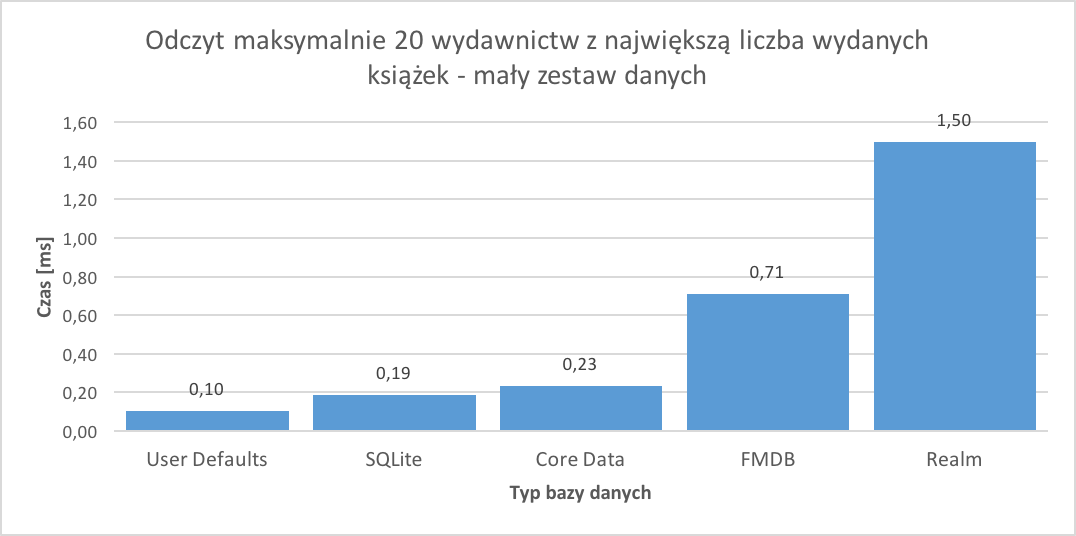
\includegraphics[width=13.5cm]{img/read_data/read_by_publishers/read_by_publishers_small_test.png}
	\caption{Odczyt wydawnictw z~największą liczba wydanych książek - mały zestaw}
	\label{fig: read-by-publishers-small}
\end{figure}

\begin{figure}[H]
\centering
	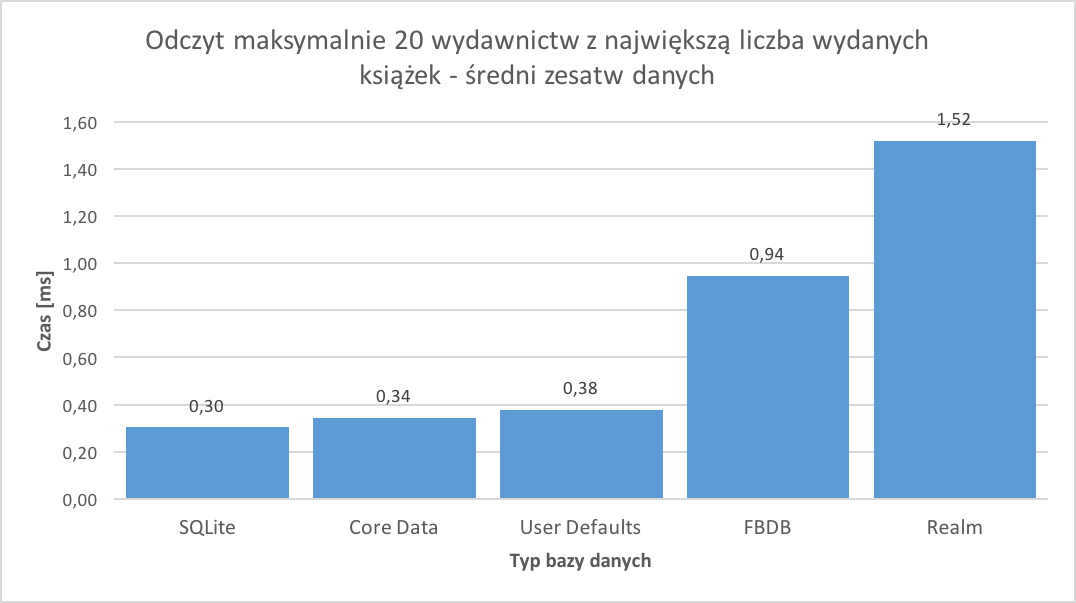
\includegraphics[width=13.5cm]{img/read_data/read_by_publishers/read_by_publishers_medium_test.png}
	\caption{Odczyt wydawnictw z~największą liczba wydanych książek - średni zestaw}
	\label{fig: read-by-publishers-medium}
\end{figure}

\begin{figure}[H]
\centering
	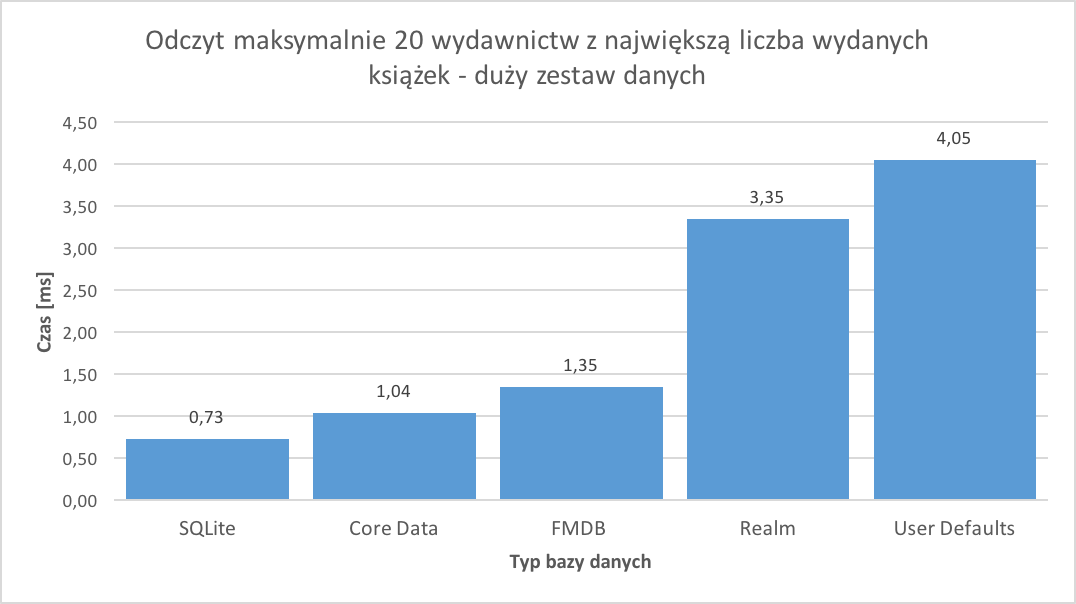
\includegraphics[width=13.5cm]{img/read_data/read_by_publishers/read_by_publishers_big_test.png}
	\caption{Odczyt wydawnictw z~największą liczba wydanych książek - duży zestaw}
	\label{fig: read-by-publishers-big}
\end{figure}

 W~przedstawionym teście zostało dodatkowo dodane sortowanie otrzymanego wyniku. Przy użyciu małego zestawu danych najszybszy czas otrzymania rezultatu uzyskała Domyślna Baza Użytkownika, skończyła wykonywać operacje w~czasie 0.10 ms. Drugi w~kolejności czas należy do SQLite i~wynosi 0.19 ms. O~0.04 ms wolniejsza okazała się Core Data, wykonując operacje w~czasie 0.23 ms. Jednym ze znacznie wolniejszych rozwiązań okazał się FMDB, uzyskał on czas 0.71 ms. Najwolniejszy w~teście okazał się Realm wykonując zadanie w~1.50 ms.\par

Przy użyciu średniego zestawu danych najszybsza jest baza SQLite, wynik otrzymany zostaje w~czasie 0.30 ms. Kolejny raz Core Data jest o~0.04 ms wolniejsza, rezultat zostaje zwrócony po 0.34 ms. Domyślna Baza Użytkownika uzyskała gorszy rezultat niż w~przypadku małego zestawu danych, uzyskała czas 0.38 ms. Przedostatnie miejsce kolejny raz zajmuje FMDB, wykonując operacje w~czasie 0.94 ms. Kolejny raz najwyższy czas należy do Realm wynosi on 1.51 ms i~jest on jedynie o~0.01 ms większy niż w~poprzednim teście.\par

Podczas testów z~wykorzystaniem największego zestawu danych najlepszy rezultat ponownie należy do SQLite, uzyskał on czas 0.73 ms. Core Data kolejny raz jest za SQLite z~czasem 1.04 ms. Lepszy wynik prezentuje FMDB, wykonując operacje odczytu w~czasie 1.35 ms. Jednym z~wolniejszych rozwiązań jest Realm, zakończenie odczytu nastąpiło w~czasie 3.35 ms. Najwolniejsza jest Domyślna Baza Użytkownika kończąc operacje w~czasie 4.05 ms. 

Prezentowane wyniki pokazują, że w~przypadku małej ilości danych w~tego typu operacji dobrze spisuję się Domyślna Baza Użytkownika lecz traci ona swoją wydajność w~przypadku dużych ilości danych. Przy większej ilości danych i~dodatkowych operacjach takich jak sortowanie wyniku znacznie lepiej spisują się rozwiązania SQL (SQLite i~FMDB) a~także Core Data. Dokumentowa baza Realm okazała się najmniej wydajna w~przedstawionym teście. 

\subsection{Testy usuwania danych}

Podrozdział przedstawia testy usuwania danych w~kilku różnych scenariuszach: 

\begin{itemize}
\item Usunięcie wszystkich danych.
\item Usunięcie wszystkich autorów którzy wydali 3 książki.
\item Usunięcie wydawnictw które wydały książki o~tytułach "Annie Oakley" lub "Tokyo Zombie (Tky zonbi)".
\end{itemize}

Testu usuwania danych przedstawiają różne stopnie skomplikowania operacji. Usunięcie wszystkich danych jest standardowym czyszczeniem bazy danych podczas którego czyszczone są wszystkie rekordy we wszystkich tablicach. Usunięcie wszystkich autorów którzy wydali 3 książki jest to operacja wymagająca zliczenia książek i~wybraniu odpowiednich rekordów do usunięcia. Usunięcie wydawnictw które wydały książki o~tytułach "Annie Oakley" lub "Tokyo Zombie (Tky zonbi)" wymaga przeszukania relacji jeden do wielu wydawnictwo - książka, porównaniu nazw i~usunięciu odpowiednich rekordów z~tablicy wydawnictwo. 

\subsubsection{Usunięcie wszystkich danych}

\begin{figure}[H]
\centering
	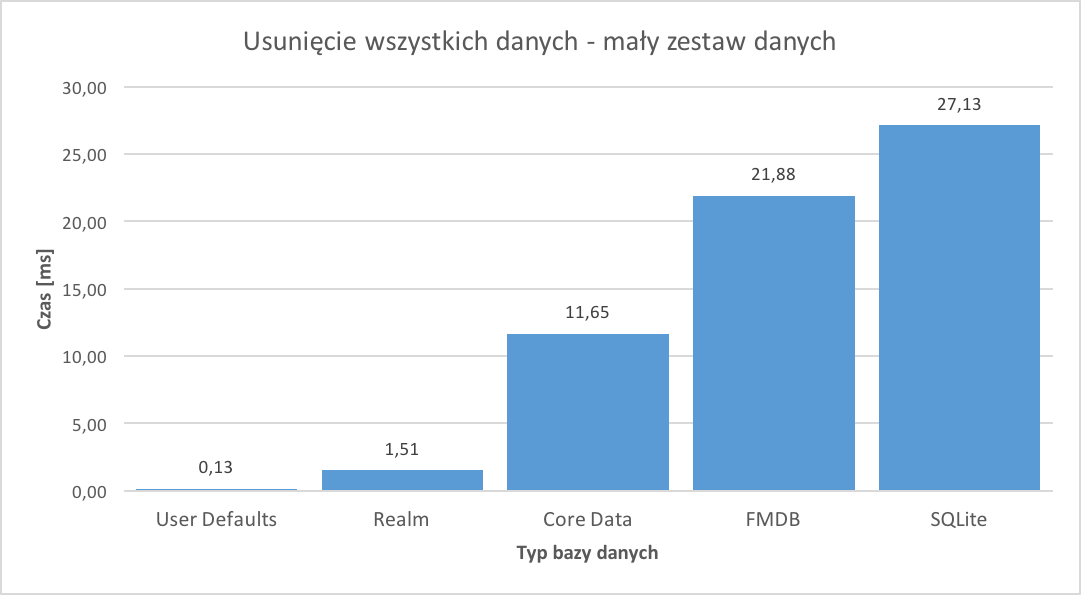
\includegraphics[width=15cm]{img/delete_data/delete_all/delete_all_small_test.png}
	\caption{Usunięcie wszystkich danych - mały zestaw}
	\label{fig: delete-all-small}
\end{figure}

\begin{figure}[H]
\centering
	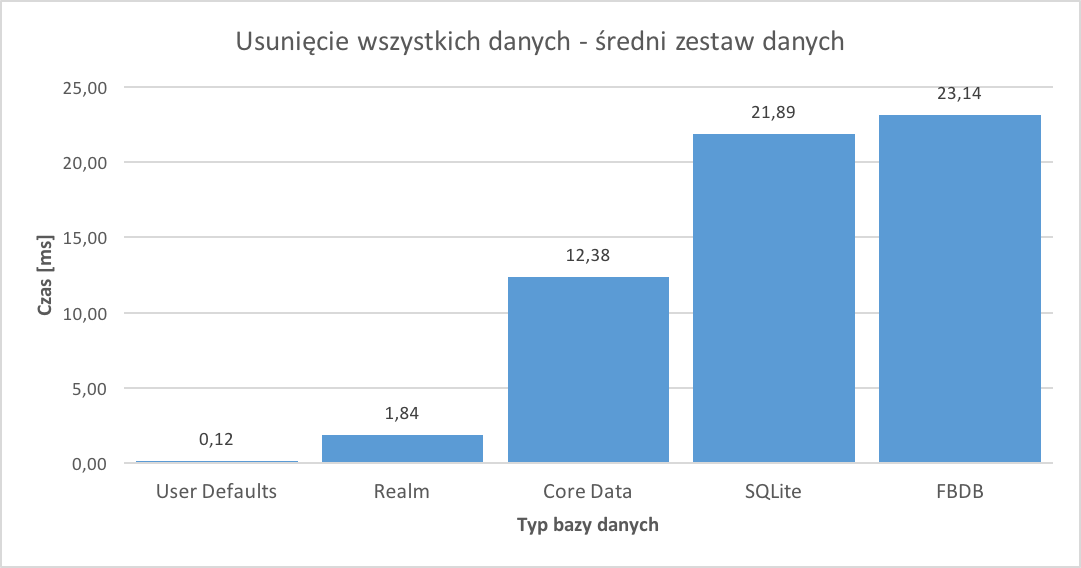
\includegraphics[width=15cm]{img/delete_data/delete_all/delete_all_medium_test.png}
	\caption{Usunięcie wszystkich danych- średni zestaw}
	\label{fig: delete-all-medium}
\end{figure}

\begin{figure}[H]
\centering
	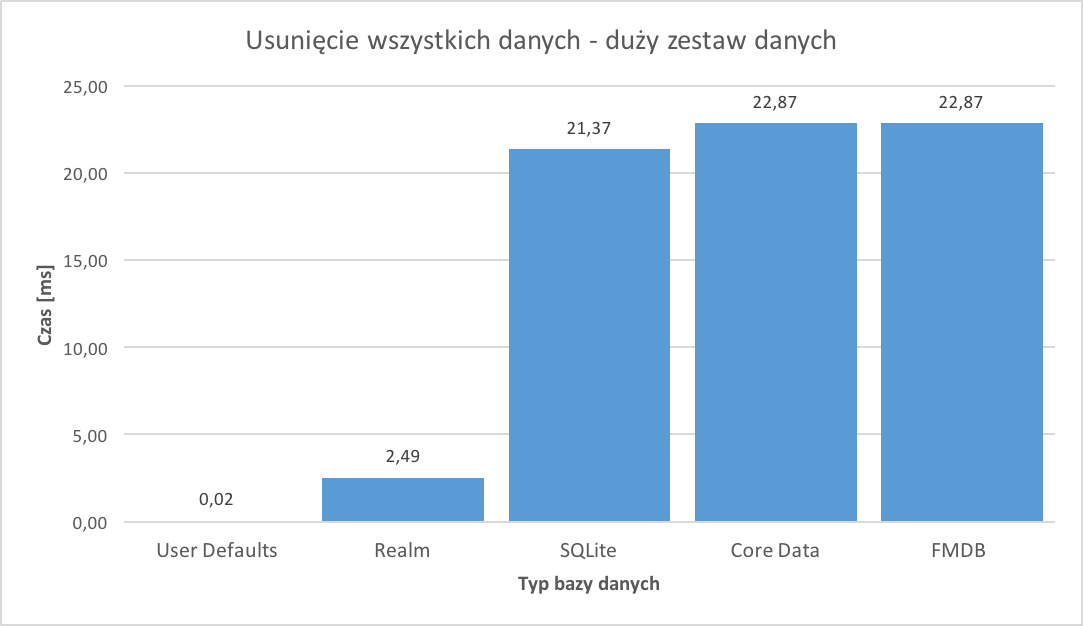
\includegraphics[width=15cm]{img/delete_data/delete_all/delete_all_big_test.png}
	\caption{Usunięcie wszystkich danych - duży zestaw}
	\label{fig: delete-all-big}
\end{figure}

Usunięcie wszystkich danych przy małym zestawie danych pokazuje, że najszybsza jest Domyślna Baza Użytkownika operacja zakończyła się po 0.13 ms. Realm uzyskał drugi czas wynoszący 1.51 ms. Core Data uzyskała rezultat znacznie wyższy od poprzednich dwóch baz danych i~usunęła dane w~czasie 11.65 ms. Najgorzej wypadły bazy SQL, FMDB wyczyścił tablice w~czasie 21.88 ms. Najwolniejszy był SQLite uzyskując czas 27.13 ms. 

Test przeprowadzony na średnim zestawie danych kolejny raz pokazuję, że najszybsza jest Domyślna Baza Użytkownika uzyskała ona czas 0.12 ms. Drugi czas ponownie osiąga Realm i~jest on równy 1.84 ms. Core Data także w~tym teście znacząco wolniej usuwa dane, czas wyniósł 12.38 ms. SQLite wraz ze wzrostem ilości danych osiągnął rezultat lepszy niż w~poprzednim teście i~ukończył operacje w~21.89 ms. Najwolniejszy tym razem jest FMDB uzyskując czas 23.14 ms. 

 W~przypadku dużego zestawu danych ponownie najlepszy rezultat należy do Domyślnej Bazy Użytkownika wynosi on 0.02 ms. Ponownie też Realm jest na drugim miejscu uzyskując czas 2.49 ms. SQLite w~porównaniu do poprzedniego testu wykonał operacje szybciej pomimo większej ilości danych. Czas uzyskany przez SQLite wynosi 21.37 i~jest o~0.51 mniejszy niż przy użyciu średniego zestawu danych. Różnica ta wynika z~obecnego stanu urządzenia, można więc przyjąć, że operacja wykonana została w~takim samym czasie. Core Data i~FMDB uzyskały takie same czasy wynoszące 22.87 ms. 

Test pokazuje, że niezależnie od zestawu danych najszybsza podczas usuwania wszystkich danych jest Domyślna Baza Użytkownika. Szybki jest też Realm jego czasy w~stosunku do zwiększającej się ilości danych nie rosną znacząco. SQLite ponownie pokazuję, że doskonale radzi sobie podczas dużej ilości danych, zaś jego wydajność podczas niewielkiej ilości rekordów nie jest zadowalająca. Rezultaty Core Data są zależne od ilości danych i~wydajność bazy spada wraz ze wzrostem ilości rekordów. Najwolniejszy w~teście okazał się wraper FMDB, zaprezentował on najmniejszą wydajność podczas testów. 

\subsubsection{Usunięcie wszystkich autorów którzy wydali 3 książki}

\begin{figure}[H]
    \centering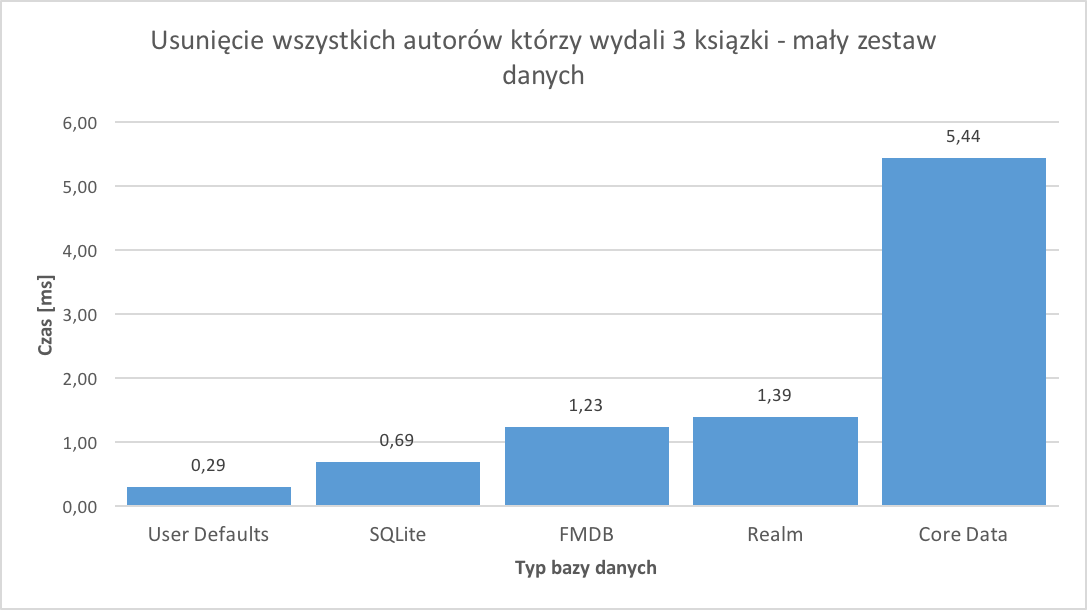
\includegraphics[width=\linewidth]{img/delete_data/delete_by_author/delete_by_author_small_test.png}
    \caption{Usunięcie wszystkich autorów którzy wydali 3 książki - mały zestaw danych}
    \label{img: delete-by-author-small}
\end{figure}

\begin{figure}[H]
    \centering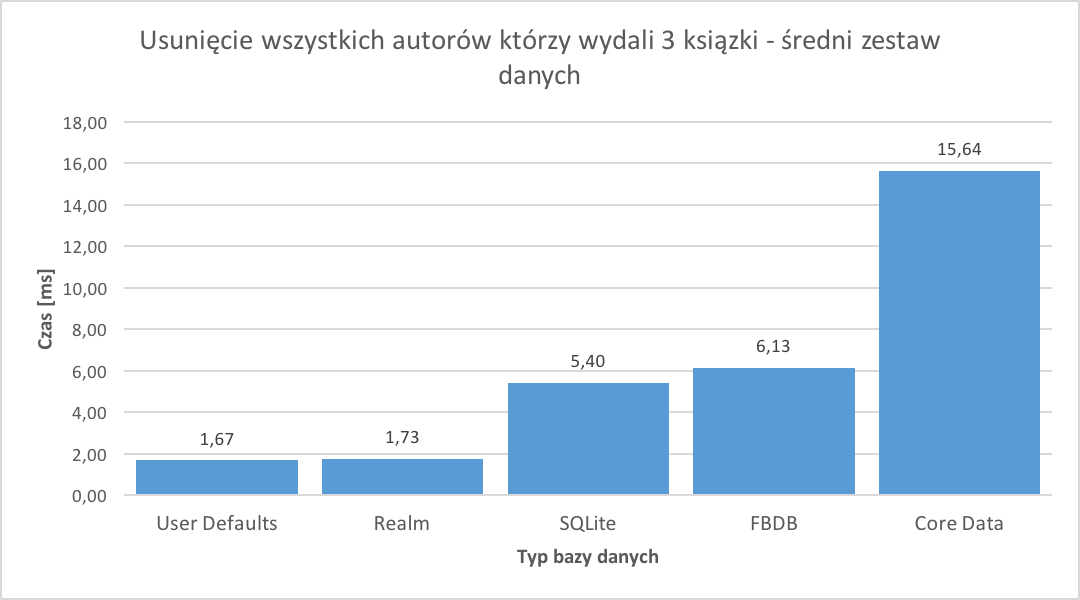
\includegraphics[width=\linewidth]{img/delete_data/delete_by_author/delete_by_author_medium_test.png}
    \caption{Usunięcie wszystkich autorów którzy wydali 3 książki - średni zestaw danych}
    \label{img: delete-by-author-medium}
\end{figure}

\begin{figure}[H]
    \centering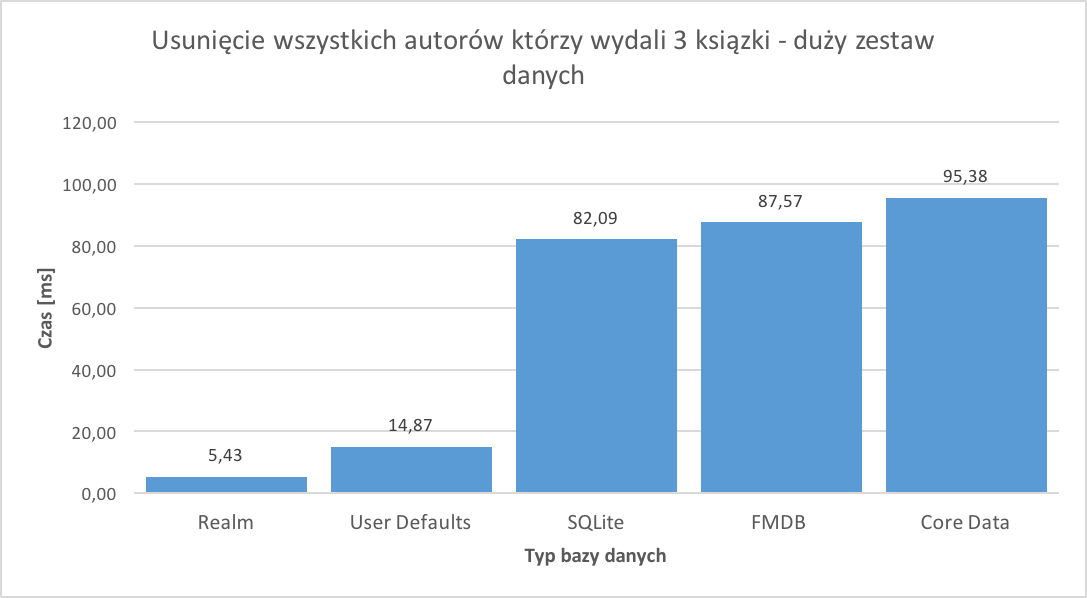
\includegraphics[width=\linewidth]{img/delete_data/delete_by_author/delete_by_author_big_test.png}
    \caption{Usunięcie wszystkich autorów którzy wydali 3 książki - duży zestaw danych}
    \label{img: delete-by-author-big}
\end{figure}

Wyniki testów usunięcie wszystkich autorów którzy wydali 3 książki w~przypadku użycia małego zestawu danych widoczne są na wykresie \ref{img: delete-by-author-small}.  Najniższy czas wynoszący 0.29 ms uzyskała Domyślna Baza Użytkownika. Drugi co do wielkości czas należy do SQLite, który uzyskał 0.69 ms. FMDB uzyskał blisko dwukrotnie wyższy czas wynoszący 1.23 ms. Realm zaś ukończył operacje z~czasem gorszym o~0.16 ms od FMDB równym 1.39 ms. Najwolniejsza okazała się Core Data, wykonała ona operacje po upływie 5.44 ms. 

Wyniki testów z~użyciem średniego zestawu danych widoczne są na wykresie \ref{img: delete-by-author-medium}. Najniższy czas równy 1.67 ms ponownie uzyskała Domyślna Baza Użytkownika. Wolniejszy o~0.06 ms okazał się Realm kończąc zadanie w~czasie 1.73 ms. SQLite zakończył operacje w~czasie 5.40 ms. FMDB zakończyło zadanie w~czasie 6.13 ms. Najwolniejsza ponownie była Core Data uzyskując czas 15.64 ms.

Rezultaty testów z~wykorzystaniem dużego zestawu danych widoczne są na wykresie \ref{img: delete-by-author-big}. Najszybszy okazał się Realm uzyskując czas 5.43 ms. Drugi co do wielkości rezultat wynoszący 14.87 ms należy do Domyślnej Bazy Użytkownika. SQlite ukończył wykonywanie zadanie w~82.09 ms. FMDB okazał się wolniejszy od SQLite o~5.48 ms i~wykonał operacje w~87.57 ms. Ponownie najwolniejsza okazała się Core Data uzyskując czas 95.38 ms.

Przedstawiony test wymagał zliczenia wszystkich książek dla każdego z~autorów a~następnie wybraniu tych, którzy wydali trzy książki i~usunięciu ich z~bazy. Wyniki pokazują że przy małej i~średniej ilości danych w~tego typu operacjach dobrze spisuję się Domyślna Baza Użytkownika, która radzi sobie gorzej w~przypadku dużej ilości danych. Realm w~przypadku małej i~średniej ilości danych wykonuję zadanie w~podobnym czasie różnica wynosi jedynie 0.34 ms, zaś ta baza danych prezentuje doskonały rezultat w~przypadku dużej ilości danych i~jest najszybsza z~testowanych baz. SQLite i~FMDB nie pokazują zaskakującej wydajności w~tego typu operacjach. FMDB przy użyciu różnych zestawów danych zawsze wypada gorzej od SQLite. Core Data okazała się najwolniejszym rozwiązaniem.

\subsubsection{Usunięcie wydawnictw które wydały książki o~tytułach ,,Annie Oakley'' lub ,,Tokyo Zombie (Tky zonbi)''}

\begin{figure}[H]
    \centering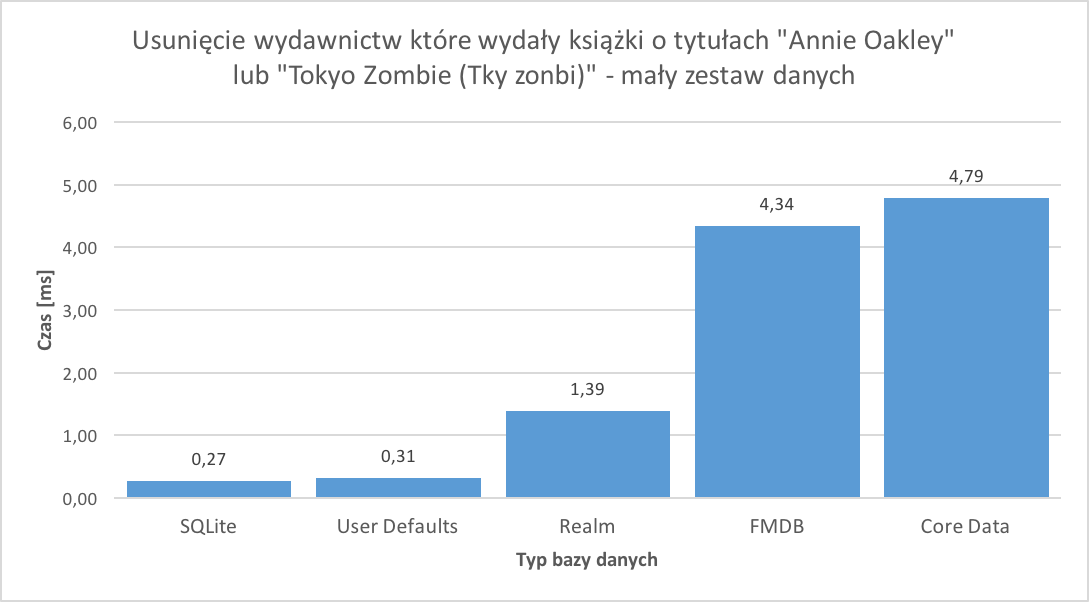
\includegraphics[width=\linewidth]{img/delete_data/delete_by_publisher/delete_by_publisher_small_test.png}
    \caption{Usunięcie wydawnictw które wydały książki o~tytułach ,,Annie Oakley'' lub ,,Tokyo Zombie (Tky zonbi)'' - mały zestaw danych}
    \label{img: delete-by-publisher-small}
\end{figure}

\begin{figure}[H]
    \centering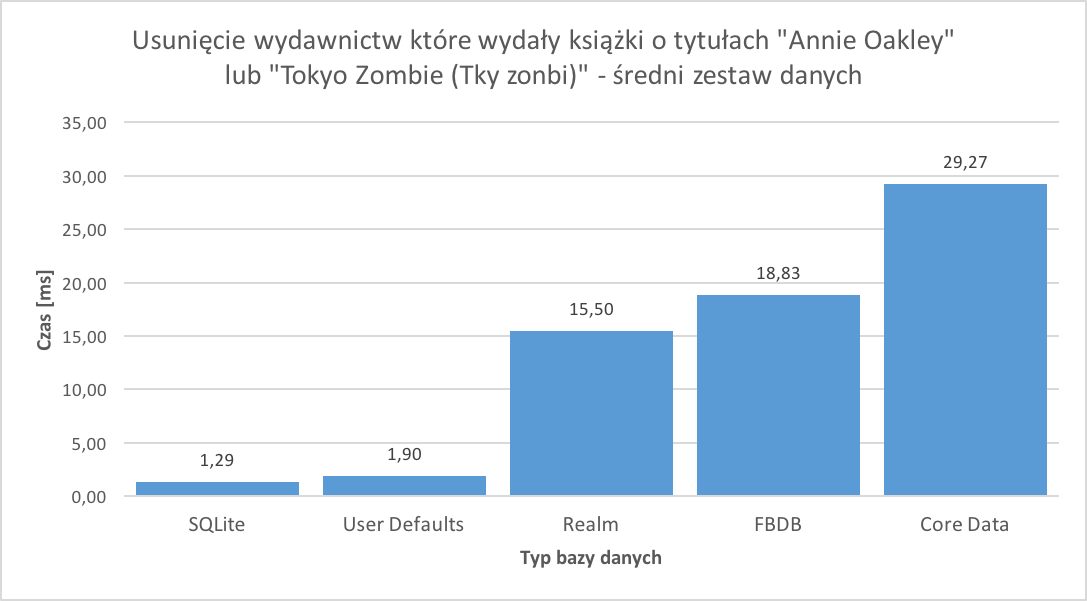
\includegraphics[width=\linewidth]{img/delete_data/delete_by_publisher/delete_by_publisher_medium_test.png}
    \caption{Usunięcie wydawnictw które wydały książki o~tytułach ,,Annie Oakley'' lub ,,Tokyo Zombie (Tky zonbi)'' - średni zestaw danych}
    \label{img: delete-by-publisher-medium}
\end{figure}

\begin{figure}[H]
    \centering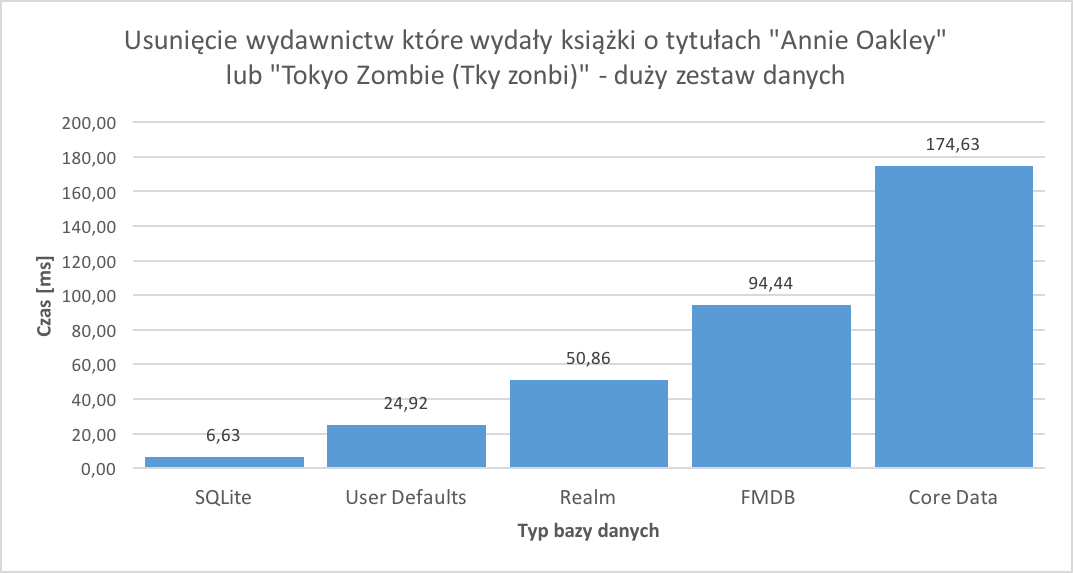
\includegraphics[width=\linewidth]{img/delete_data/delete_by_publisher/delete_by_publisher_big_test.png}
    \caption{Usunięcie wydawnictw które wydały książki o~tytułach ,,Annie Oakley'' lub ,,Tokyo Zombie (Tky zonbi)'' - duży zestaw danych}
    \label{img: delete-by-publisher-big}
\end{figure}

Rezultaty testu usunięcia wydawnictw które wydały książki o~tytułach ,,Annie Oakley'' lub ,,Tokyo Zombie (Tky zonbi)'' z~użyciem małego zestawu danych widoczne na wykresie \ref{img: delete-by-publisher-small} pokazują, że najszybszy w~tym przypadku okazał się SQLite. Uzyskał on czas równy 0.27 ms. Wolniej wykonała operacje Domyślna Baza Użytkownika kończąc zadanie w~ciągu 0.31 ms. Trzeci rezultat uzyskał Realm wykonując operacje w~1.39 ms. FMDB ukończył zadanie w~4.34 ms, zaś Core Data okazała się najwolniejsza czas zakończenia operacji w~jej wykonaniu wyniósł 4.79 ms. 

 W~przypadku średniego zestawu danych ponownie najszybszy jest SQLite z~czasem 1.29 ms. Ponownie nieznacznie wolniejsza w~stosunku do SQLite okazała się Domyślna Baza Użytkownika wykonując operacje w~1.90 ms. Realm przedstawia znaczny spadek wydajności względem poprzedników kończąc zadanie po upływie 15.50 ms co jest o~13.9 ms wolniej niż Domyślna Baza Użytkownika. FMDB i~Core Data ponowni okazały się najmniej wydajne. Czas wykonania testu dla FMDB wynosi 18.83 ms zaś dla Core Data równy jest on 29.27 ms.

Podczas wykorzystania dużego zestawu danych kolejność uzyskanych czasów przez bazy nie uległa zmianie. Ponownie najszybszy jest SQLite, czas wyniósł 6.63 ms. Znacznie wolniej operacje wykonała Domyślna Baza Użytkownika, zadanie wykonane zostało po upływie 24.92 ms. Realm zakończył operacje w~50.86 ms. FMDB zakończył usuwanie wybranych wydawnictwa w~czasie 94.44 ms. Core Data prezentuje znacznie wolniejsze działanie w~tego typu zapytaniach, uzyskała największy czas równy 174.6 ms. 

Test pokazuję, że w~przypadku operacji wymagającej pracy z~relacjami pomiędzy danymi najszybszym rozwiązaniem jest SQLite. Domyślna Baza Użytkownika ponownie prezentuje duży spadek wydajności wraz ze wzrostem ilości danych. Realm i~FMDB prezentują zbliżone wyniki lecz kiedy operacje wykonywane są na dużej ilości danych zdecydowaną przewagę posiada Realm. Core Data niezależnie od ilości danych posiada najmniejszą wydajność z~pośród testowanych baz danych niezależnie od ilości danych.

\subsection{Testy edycji danych}

Podrozdział przedstawia testy edycji danych w~dwóch różnych opcjach: 

\begin{itemize}
\item Zmiana imienia autora ,,Diena'' na ,,Alona''.
\item Zmiana daty wydania książek na obecna datę.
\end{itemize}

Pierwszy z~testów przedstawia operacje przeprowadzoną na wybranych rekordach z~tabeli, wymaga on przeszukania bazy w~celu odnalezienia odpowiedniego rekordu do edycji. Drugi test jest operacją przeprowadzaną na całej tablicy bez potrzeby wykonywania dodatkowych operacji wyszukiwania w~obrębie danego rekordu.

\subsubsection{Zmiana imienia autora ,,Diena'' na ,,Alona''}

\begin{figure}[H]
    \centering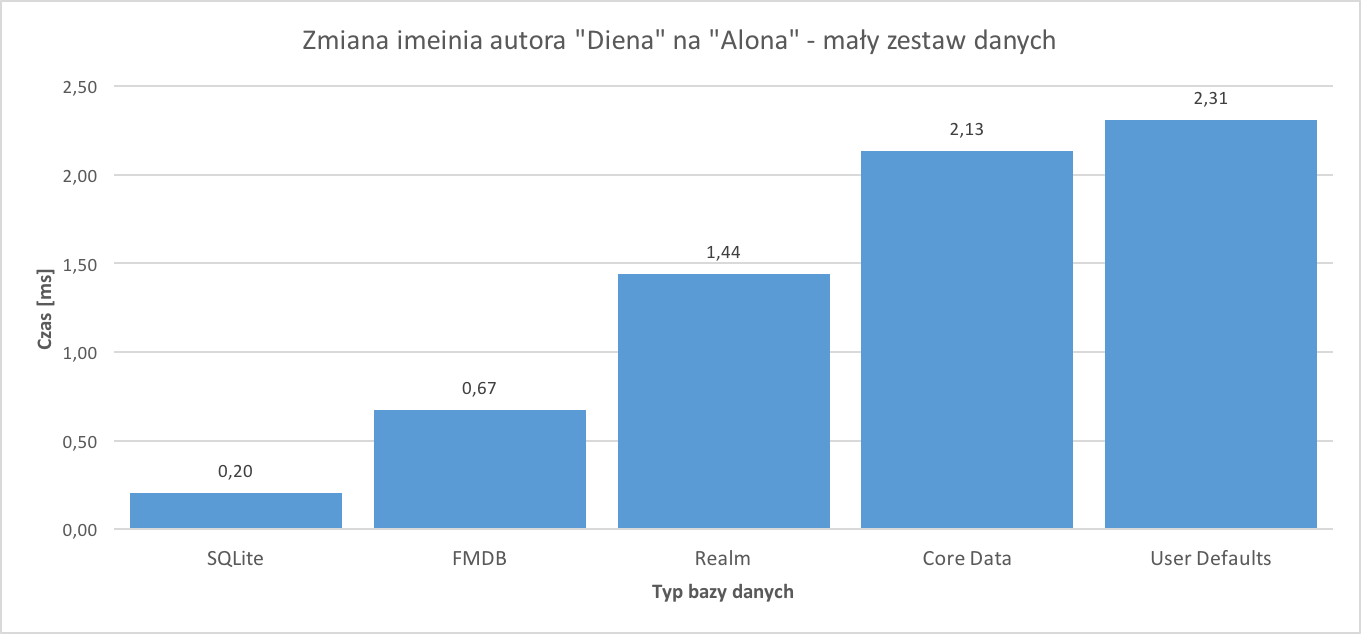
\includegraphics[width=\linewidth]{img/update_data/update_author/update_author_small_test.png}
    \caption{Zmiana imienia autora ,,Diena'' na ,,Alona'' - mały zestaw danych}
    \label{img: update-by-author-small}
\end{figure}

\begin{figure}[H]
    \centering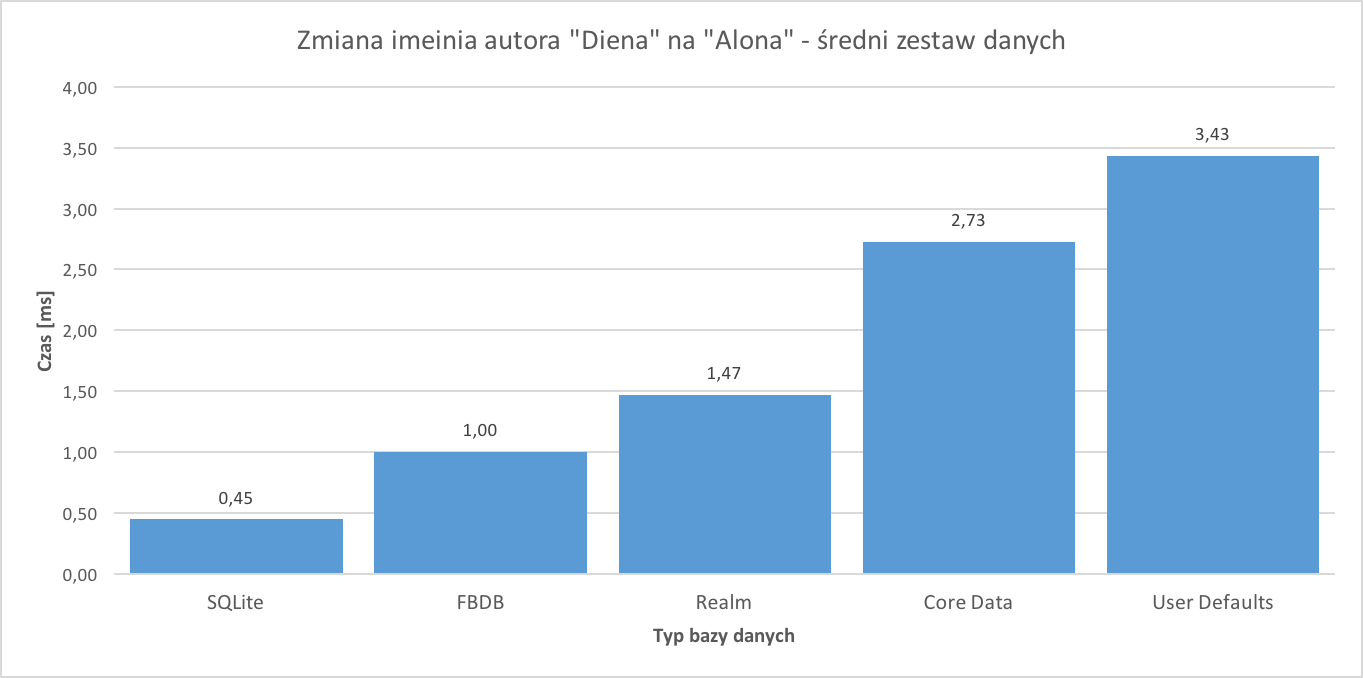
\includegraphics[width=\linewidth]{img/update_data/update_author/update_author_medium_test.png}
    \caption{Zmiana imienia autora ,,Diena'' na ,,Alona'' - średni zestaw danych}
    \label{img: update-by-author-medium}
\end{figure}

\begin{figure}[H]
    \centering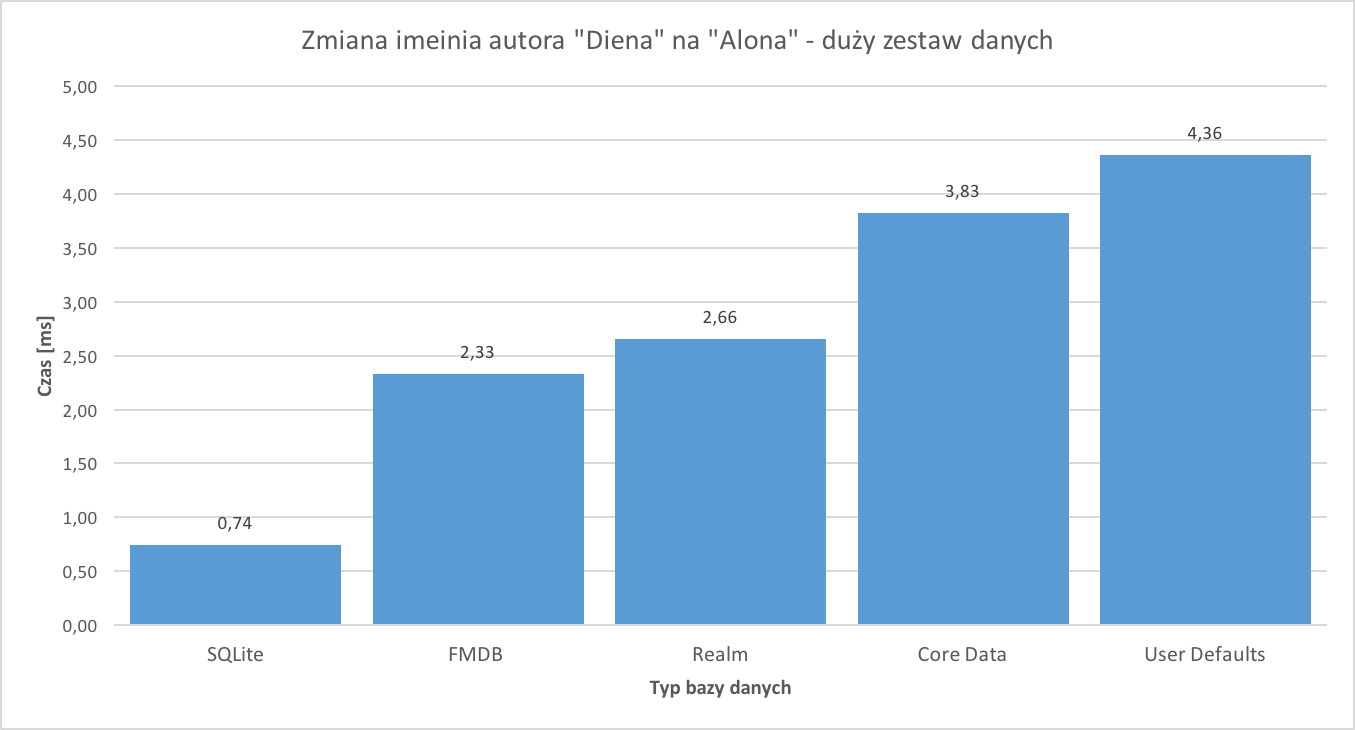
\includegraphics[width=\linewidth]{img/update_data/update_author/update_author_big_test.png}
    \caption{Zmiana imienia autora ,,Diena'' na ,,Alona'' - duży zestaw danych}
    \label{img: update-by-author-big}
\end{figure}

Test zmiany imienia autora ,,Diena'' na ,,Alona'' z~użyciem małego zestawu danych najszybciej wykonał SQLite uzyskując czas 0.20 ms. Wraper FMDB zakończył to zadanie w~czasie 0.67 ms. Realm test zakończył po upływie 1.44 ms. Core Data pokazała niższa wydajność i~skończyła zadanie w~czasie 2.13 ms. Najwolniejsza okazała się Domyślna Baza Użytkownika kończąc operacje w~czasie 2.31 ms. 

Zastosowanie średniego zestawu danych przyniosło następujące rezultaty. SQLite wykonał operacje w~czasie 0.45 ms. FMDB okazał się wolniejszy o~0.55 ms i~uzyskał czas 1 ms. Dla bazy Realm test zajął 1.47 ms. Core Data zakończyła zadanie w~czasie 2.73 ms. Ponownie najmniej wydajna jest Domyślna Baza Użytkownika kończąc test w~3.43 ms.

Użycie dużego zestawu danych pokazuje, że SQLite w~dalszym ciągu jest bardzo wydajny, czas ukończenia operacji w~tym przypadku wyniósł 0.74 ms. Znacznie wolniejszy jest FMDB, zakończył test w~2.33 ms. Realm przy zwiększonej ilości danych uzyskał czas 2.66 ms zaś Core Data potrzebowała 3.83 ms na edycje danych. Domyślna Baza Użytkownika po raz kolejny była najmniej wydajna potrzebowała aż 4.36 ms aby wykonać test. 

Test pokazuję, że wybranie odpowiednich rekordów i~ich edycja jest mocną stroną baz SQL, SQLite i~FMDB pokazują największą wydajność w~wykonanym teście niezależnie od ilości danych. Pozostałe bazy danych poddane testowi zwiększają swoje czasy wraz ze wzrostem ilości danych. Najmniej wydajną bazą w~przypadku przedstawionego testu jest Domyślna Baza Użytkownika. 

\subsubsection{Zmiana daty wydania książek na obecna datę}

\begin{figure}[H]
    \centering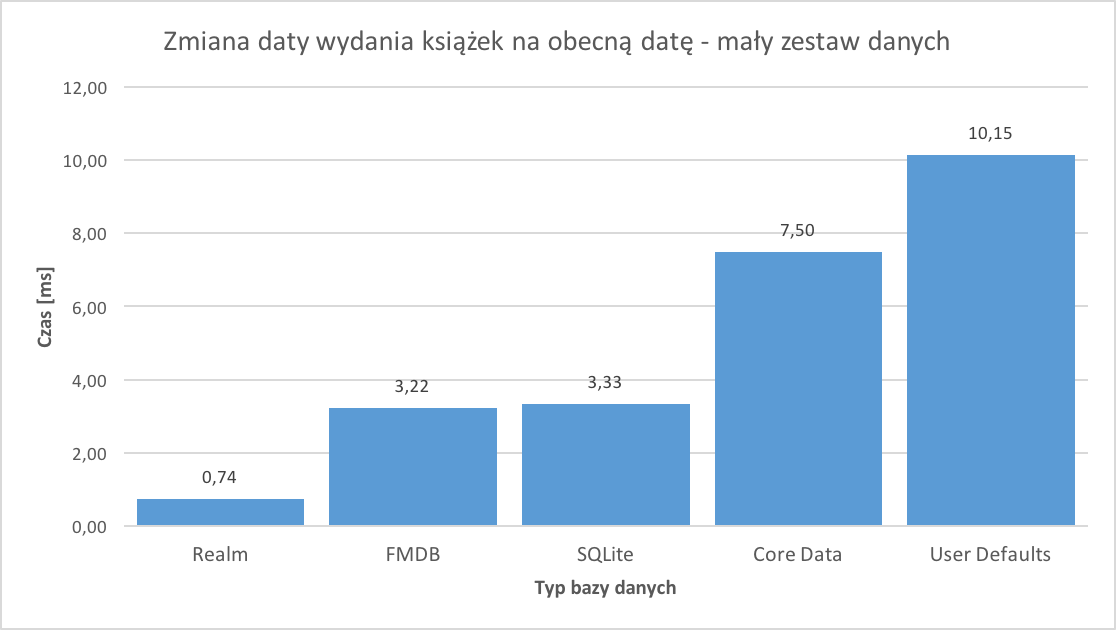
\includegraphics[width=\linewidth]{img/update_data/update_book/update_book_small_test.png}
    \caption{Zmiana daty wydania książek na obecna datę - mały zestaw danych}
    \label{img: update-by-book-small}
\end{figure}

\begin{figure}[H]
    \centering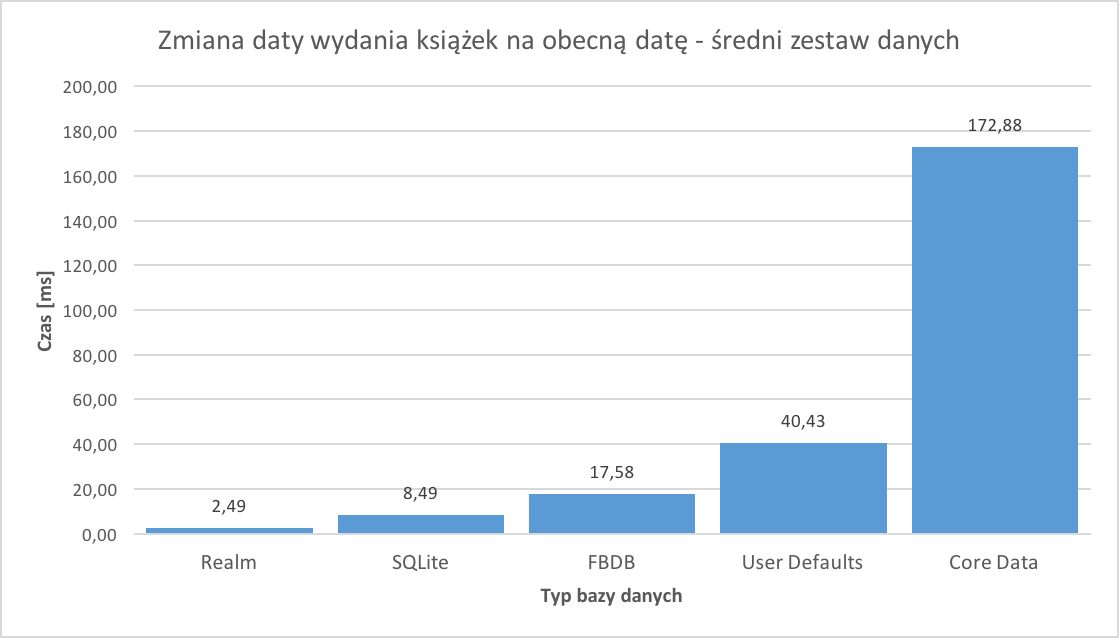
\includegraphics[width=\linewidth]{img/update_data/update_book/update_book_medium_test.png}
    \caption{Zmiana daty wydania książek na obecna datę - średni zestaw danych}
    \label{img: update-by-book-medium}
\end{figure}

\begin{figure}[H]
    \centering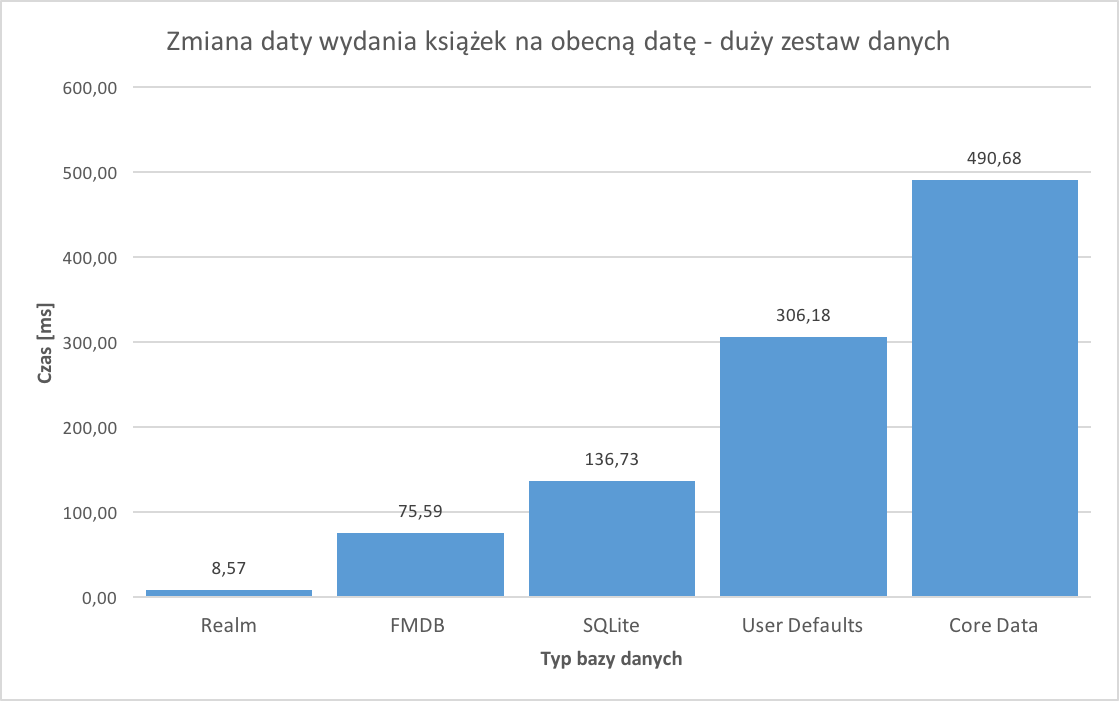
\includegraphics[width=\linewidth]{img/update_data/update_book/update_book_big_test.png}
    \caption{Zmiana daty wydania książek na obecna datę - duży zestaw danych}
    \label{img: update-by-book-big}
\end{figure}

Test zmiany daty wydania książek na obecna datę operował na wszystkich rekordach w~tabeli Książka. Rezultaty w~przypadku małego zestawu danych prezentują się następująco. Realm zakończył test w~czasie 0.74 ms. FMDB i~SQLite ukończyły operacje kolejno w~czasach 3.22 i~3.33 ms. Core Data okazała się znacznie wolniejsza od poprzedników i~potrzebowała 7.50 ms aby zakończyć zadanie. Najwolniejsza jest Domyślna Baza Użytkownika uzyskując czas wykonania operacji równy 10.15 ms. 

Średni zestaw danych w~przedstawianym teście przedstawia bardzo wysoką wydajność bazy Realm, zakończył on operacje w~2.49 ms. SQLite na wykonanie testu potrzebował 8.49 ms. FMDB zakończył zadanie w~czasie 17.58 ms. Znacznie wolniejsza od poprzednich baz jest Domyślna Baza Użytkownika, zakończyła test w~40.43 ms. Najwolniejsza jest Core Data potrzebowała aż 172.88  ms na uaktualnienie dat wydania książek.

Użycie dużego zestawu danych pokazało, że w~dalszym ciągu Realm jest w~podanym teście najszybszy, czas zakończenia operacji wyniósł 8.57 ms. Dużo wolniejszy jest FMDB potrzebował aż 75.59 ms. SQLite także potrzebował dużo czasu na zakończenie testu, operacja wymagała 136.73 ms. Domyślna Baza Użytkownika operacje zakończyła po upływie 306.18 ms. Core Data na wykonanie testu potrzebowała 490,68 ms. 

Podczas edycji każdego z~rekordów tabeli najwydajniejszą bazą okazał się Realm. Wolniejsze od dokumentowej bazy danych okazały się bazy SQL, edycja danych zajęła im więcej czasu. Najmniej wydajna jest Domyślna Baza Użytkownika oraz Core Data, której wydajność jest bardzo słaba w~przedstawionej operacji. 